% draft 3rd year diploma thesis, by Nick Manini, 2013/03/22
\documentclass[a4paper,12pt]{article}
\usepackage[english]{babel} % or other languages, e.g:
%\usepackage[italian]{babel} % needs debian package texlive-lang-italian
%\usepackage[latin1]{inputenc} % use to reproduce accented characters correctly
\usepackage{hyperref}
\usepackage{graphicx}
\usepackage{amsmath}
\usepackage{amssymb}
\usepackage{physics}
\usepackage{enumitem}
\usepackage{framed}
\usepackage[width=125mm]{caption}

\graphicspath{{./media/images/}}

\usepackage[document]{ragged2e}
\usepackage{verbatim}

\usepackage{fancyhdr}
\pagestyle{fancy}
\fancyhead[LE,RO]{\slshape}
\fancyfoot[C]{\thepage}

%include the git footer with the last commit
\include{gitfooter}

% Dimensione della pagina
\setlength{\oddsidemargin}{.3in}  % Distance from the left edge -1 inch 
\setlength{\textwidth}{145mm}     % Normal width of the text
\setlength{\topmargin}{.25in}     % Distance from top to PAGE'S HEAD -1 inch
\setlength{\textheight}{225mm}    % Height of the body of page
\setlength{\headheight}{0mm}      % Height of a box containing the head
\setlength{\parskip}{0.5mm}         % Extra vertical space before a paragraph
\setlength{\parindent}{9mm}       % Width of the indentation 
\linespread{1.12}                 % Line spacing        
\renewcommand{\floatpagefraction}{.9}

\usepackage{xcolor}
\newcommand\mynotes[1]{\begin{flushright}

\textcolor{red}{TODO: #1}\end{flushright}}
\newcommand{\jsqrt}[2]{\bqty{ #1 #1 | #2 #2 }}
\newcommand{\ksqrt}[2]{\bqty{ #1 #2 | #2 #1 }}
\newcommand\mf[1]{\mathbf{#1}}
\newcommand\dens{\rho(\mathbf{r})}
\newcommand\densin{\rho^{in}(\mathbf{r})}
\newcommand\densout{\rho^{out}(\mathbf{r})}
\newcommand\rdens{\tilde{\rho}(\mathbf{G})}
\newcommand\erre{\mathbf{r}}
\newcommand\GI{\mathbf{G}}
\newcommand\QE{\textsc{Quantum} ESPRESSO }
\newcommand\numbands{n_{bands}}
\newcommand\numG{n_{G}}
\newcommand\numR{n_{R}}
\newcommand\bigO{\mathcal{O}}
\newcommand\CO{CO3 } 
%nome del sistema CO3

\begin{document}

\title{\bf \Huge Tuning the computational architecture for Quantum Espresso ab initio calculation of nanostructures }


\author{Giorgio Ruffa\\
Dipartimento di Fisica, Universit\`a degli Studi di Milano,\\
Via Celoria 16, 20133 Milano, Italia
}
\date{April 22, 2016} % the exact date of graduation, when available


{
\thispagestyle{empty}

\centerline{

\includegraphics[width=120mm,angle=0,clip=]{UniversitasMediolanensis.eps}
}

\begin{center}
{\Large Facolt\`a di Scienze e Tecnologie\\
\vskip0.2cm Laurea Triennale in Fisica }
\end{center}


\vskip1.5cm
\begin{center}
{\huge \textbf{Titolazzo della tesi, if seems long\\go to newline}}
\end{center}

{\large
\vskip20mm Relatore:  Prof. Dario Tamascelli
\vskip 1mm Correlatore: Prof. Michele Ceotto\\
\vskip 1mm Relatore Esterno: Dott. Davide Ceresoli\\
}

\vskip2cm
\hskip9cm\parbox[t]{7cm}
{\large 
Giorgio Ruffa\\
Matricola n$^\circ$ $742031$\\
A.A. $2015$/$2016$\\
\vskip 0.5mm Codice PACS: ?9.?a.?Z
}

\newpage
\newpage
\thispagestyle{empty}
\clearpage
}

 % eccezionalmente qui include il frontespizio
% in general avoid \include altoghether, it is looking for trouble !!

\newpage\qquad
\newpage

\maketitle

%---------------------------------------------------------
\begin{abstract}

Quantum Espresso (QE) is one of the most reliable and widespread  suite of codes for quantum chemistry calculations of nanostructures. Given the relevance of QE for the condensed matter physics community, we perform a detailed analysis of the information flow within the QE codes. We undertake several nanostructure systems to highlight how the computational data flow is related to the geometry and to the dimensionality of the nanostructures. These tests are performed on different computer architectures as to determine how the memory access type impacts the overall performance of the code.

\vskip0.75cm
\hskip5cm
\parbox[t]{7cm}
{
Advisor: {\it Dott. Dario Tamascelli}\\
Co-Advisor: {\it Prof. Michele Ceotto}\\
External Advisor: {\it Dott. Davide Ceresoli}\\
}
\end{abstract}
%--------------------------------------------------------

\newpage
\tableofcontents
\newpage


\section{Ab Initio calculations in modern Solid State Physics}
\mynotes{importanza dei conti nel calcula delle strutture elettroniche}


\section{Theoretical Introduction}\label{model:sec}

This section will cover the basic theory upon which Quantum ESPRESSO is based.

By starting with a very general approach we can say that the Hamiltonian associated to a system of atoms with $N_N$ nuclei and $N_e$ electrons can be written as:


\begin{equation}\label{eq:theHamiltonianLong}
\hat{H}_{tot} = \hat{T}_{N} + \hat{T}_{e} + \hat{V}_{Ne} + \hat{V}_{NN} + \hat{V}_{ee}.
\end{equation}

Where:

\begin{equation}
\hat{T}_{N} = - \frac{\hbar}{2} \sum_{\alpha}^{N_N} \frac{\nabla_{\alpha}^2}{M_{\alpha}},
\end{equation}
is the kinetic energy of the nuclei.

\begin{equation}
\hat{T}_{e} = - \frac{\hbar}{2m_{e}} \sum_{i}^{N_e} \nabla_{i}^2,
\end{equation}
is the kinetic energy of the electrons.

\begin{equation}
\hat{V}_{Ne} = -\frac{e^2}{4\pi\varepsilon_{0}} \sum_{i}^{N_e}\sum_{\alpha}^{N_N} \frac{Z_{\alpha}}{\mid R_{\alpha} - r_{i} \mid },
\end{equation}
is the electron-ion attraction potential energy.

\begin{equation}
\hat{V}_{NN} = \frac{e^2}{4\pi\varepsilon_{0}} \frac{1}{2} \sum_{\alpha \neq \beta}^{N_N} \frac{Z_{\alpha} Z_{\beta}}{\mid R_{\alpha} - R_{\beta} \mid },
\end{equation}
is the nucleus-nucleus repulsion potential energy.

\begin{equation}
\hat{V}_{ee} = \frac{e^2}{4\pi\varepsilon_{0}} \frac{1}{2} \sum_{i \neq j}^{N_e} \frac{1}{\mid r_{i} - r_{j} \mid },
\end{equation}
is the electron-electron repulsion potential energy.

A state function $\ket{\psi}$ describing all the particles involved in the system will evolve following the Schr\"odinger equation
\begin{equation}\label{eq:eq_sch}
	i\hbar\dv{t}\ket{\psi(t)} = \hat{H}_{tot}\ket{\psi(t)}.
\end{equation}

From now on, if not explicitly specified, we will use atomic units \footnote{see \cite[p.42]{Attila} for further details}
\begin{equation}
	m_{e} = \hbar = e =\frac{1}{4 \pi \epsilon_{0}} = 1.
\end{equation}

We shall rewrite equation \eqref{eq:theHamiltonianLong} in a much more elegant form:


\begin{equation}\label{eq:theHamiltonian}
\boxed{
	\hat{H}_{tot}   = - \sum_{\alpha}^{N_N} \frac{\nabla^2_{\alpha}}{2M_{\alpha}}
					+ \frac{1}{2}\sum_{\alpha \neq \beta}^{N_N} \frac{Z_{\alpha} Z_{\beta}} {R_{\alpha \beta}}
					- \sum_{i}^{N_e} \frac{\nabla_{i}^2}{2}
					- \sum_{i}^{N_e} \sum_{\alpha}^{N_N} \frac{ Z_{\alpha} }{r_{i \alpha}}				
					+ \frac{1}{2} \sum_{i \neq j}^{N_e} \frac{1}{r_{ij}}
,}
\end{equation}
with:
\begin{align*}
	r_{ij} & = \mid r_{i} - r_{j} \mid ;
\\
	r_{i \alpha} & = \mid r_{i} - R_{\alpha} \mid ;
\\
	R_{\alpha \beta} & = \mid R_{\alpha} - R_{\beta} \mid .
\end{align*}

Although the universality of this equation\footnote{It must be noted that we are neglecting any relativistic effect.}, we know very well that even a simple molecule like $H_2^{+}$ has no analytical solution.

Thus, even from a computational standpoint, a set of approximations must be performed.


\subsection{The Born-Oppenheimer Approximation}

The Born-Oppenheimer approximation takes note of the great difference in masses of electrons and nuclei.
Nuclear mass is much higher than electron mass, so we expect electrons to have much higher velocities than	 nuclei. 

It's now reasonable to separate the motion of the system in two distinct movements: the \textit{``slow"} movement of the nuclei, and the \textit{``fast"} movement of the electrons.

We can say that from the point of view of electrons, the nuclei appear to be fixed. 
From a physical standpoint the electrons are moving in the static field produced by the nuclei while still interacting within each others \cite[p.241]{Atkins}.


Using this approximation the kinetic energy of the nuclei $\hat{T}_{NN}$ can be neglected and the repulsion between the nuclei $\hat{V}_{NN}$, can be considered to be constant.

We will consider now the electronic Hamiltonian $H_{elec}$ :
\begin{equation}
	\hat{H}_{e} = \hat{T}_{e} + \hat{V}_{Ne} + \hat{V}_{ee}
\end{equation}

Rewriting $\hat{H}_{e}$  using atomic units:
\begin{equation}\label{eq:H_elec}
	\hat{H}_{e} = 	- \sum_{i}^{N_{e}} \frac{1}{2} \nabla_{i}^2  
					- \sum_{i}^{N_{e}} \sum_{\alpha}^{N_{N}} \frac{Z_{\alpha}}{r_{i\alpha}}  
					+ \frac{1}{2} \sum_{i \neq j}^{N_{e}} \frac{1}{r_{ij}}.
\end{equation}

Then equation \eqref{eq:eq_sch} then becomes:
\begin{equation}
	\hat{H}_{e} \ket{\Phi_{e}} = \varepsilon_{e} \ket{\Phi_{e}},
\end{equation}

with solution
\begin{equation}
	\ket{\Phi_{e}} = \ket{\Phi_{e}( \{r_{i}\};\{R_{\alpha}\} )}.
\end{equation}

Where the dependency from the electronic coordinates $\{r_i\}$ is explicit, but the dependency from nuclear coordinates $\{R_{\alpha}\}$ is parametric.
This implies that also the electronic energy depends parametrically on $\{R_{\alpha}\}$

\begin{equation}
	\varepsilon_{e} = \varepsilon_{e}(\{R_{\alpha}\}).
\end{equation}

To obtain the total energy (with fixed nuclei) we have to add the constant ion-ion Coulomb potential energy

\begin{equation}\label{eq:totEn1}
	\varepsilon_{tot} = \varepsilon_{e} + \frac{1}{2} \sum_{\alpha \neq \beta}^{N_N} \frac{Z_{\alpha} Z_{\beta} }{R_{\alpha \beta}}.
\end{equation}

Equation from \eqref{eq:H_elec} to \eqref{eq:totEn1} constitutes the so called \textit{``Electronic Problem"} \cite[p.44]{Attila}.

Once solved one could then apply the same principle to the nuclear problem.
Since the electrons moves much faster then the nuclei, it is reasonable to approximate \eqref{eq:theHamiltonian} by replacing electronic coordinates by their average value, averaged over $\Phi_{e}$.
The nuclear Hamiltonian will be :
\begin{equation}
	H_{N} = - \sum_{\alpha}^{N_{\alpha}} \frac{1}{2M_{\alpha}} \nabla_{\alpha}^2 + \varepsilon_{tot}(\{ R_{\alpha}\}).
\end{equation}

We can see that $\varepsilon_{tot}(\{ R_{\alpha}\})$ is a potential energy surface for nuclear motion.

Thus the nuclei in the Born-Oppenheimer approximation move on a potential energy surface obtained by solving the electronic problem.

The nuclear Schr\"odinger equation  
\begin{equation}
	\hat{H}_{N} \ket{\Phi_{N}} = \varepsilon \ket{\Phi_{N} },
\end{equation}

with solution 

\begin{equation}
	\ket{\Phi_{N}}=\ket{\Phi_{N}(\{R_{\alpha}\})},
\end{equation}

will describe vibration, rotation, and translation of the molecule.

The complete approximate solution to \eqref{eq:theHamiltonian} will be  \cite[p.43-45]{Attila}

\begin{equation}
	\ket{ \Phi(\{r_i\};\{R_{\alpha}\}) } 	= \ket{ \Phi_{e}(\{r_i\};\{R_{\alpha}\})} 
											~ \ket{ \Phi_{N}(\{R_{\alpha}\})}.
\end{equation}

Since this work will mainly focus on the \textit{``electronic problem"}, from now on we will drop the suffix ``$e$" for the Hamiltonian $H_{e}$.

\subsection{The Hartree Product}
\subsubsection{Spin-Orbit}
We introduce two single particle spin functions  $\alpha(\omega), \beta(\omega)$, corresponding respectively to spin up and spin down.
The only conditions we impose is that these two functions are orthonormal and form a complete set of auto-functions for the spin operator $\hat{S}_z$ \footnote{Even if it isn't necessary to specify the eigenvalues of the spin operator (as stated in \cite{Attila}), we prefer to specify them since we'll deal only with fermions. }:

\begin{align*}
	\bra{\alpha}\ket{\alpha} & = \bra{\beta}\ket{\beta} = 1; \\
	\bra{\alpha}\ket{\beta} & = \bra{\beta}\ket{\alpha} = 0; \\
	\hat{S}_{z} \ket{\alpha} & = + \frac{1}{2} \ket{\alpha}; \\
	\hat{S}_{z} \ket{\beta} & = - \frac{1}{2} \ket{\beta}. \\
\end{align*}

An electron is described by three spacial coordinates $\mathbf{r}$ and one spin coordinate $\omega$
\begin{equation}
	\mathbf{x} = \{\mathbf{r},\omega\}.
\end{equation}

We define $\psi_i(\mathbf{r})$ a spacial orbital as a function of the position vector $\mathbf{r}$ describing the spacial distribution of an electron, so that $\mid\psi_i(\mathbf{r})\mid^2 {dr}^3$ is the probability of finding the electron in a small volume ${dr}^3$ centered at position $\mathbf{r}$.

Given a set of spatial orbitals we will assume them to be orthonormal, thus if the set is complete we can express any spatial state function as a linear combination of spatial orbitals.

In general, for the set to be complete, one should consider it as infinite. As one can imagine, in practice, an infinite orbitals' set is not available and we will consider only a finite set composed of $K$ such orbitals. The finite set will only cover a certain region of the complete space, but we will consider the results to be ``exact" within the subspace generated by the finite set of spatial orbitals.

The combination of a spatial orbital and a spin function is called a spin orbital and completely describes the electron
\begin{equation}
	\chi_{i}(\mathbf{x}) = \psi_i(\mathbf{r}) \alpha(\omega).
\end{equation}


For a set of K spatial orbital will have a corresponding set of $2K$ spin orbitals, each pair sharing the same spatial orbital but with different spin function:

\begin{equation}
	\chi_{2i} = \psi_i(\mathbf{r}) \alpha(\omega);
\end{equation}
\begin{equation}
	\chi_{2i-1} = \psi_i(\mathbf{r}) \beta(\omega).
\end{equation}

Being the spatial orbital and spin orbitals orthonormal, so are the spin orbitals.

\subsubsection{Separating the problem}

It is evident that the term $V_{ee}$ in \eqref{eq:H_elec} is the more complicated to handle in order to find an exact solution to the electronic problem.
To simplify the system we start by neglecting $V_{ee}$, considering the electrons as non interacting.
The Hamiltonian \eqref{eq:H_elec} can be rewritten in the following form:
\begin{align}
	\hat{H} & = \sum_{i}^{N_{e}} \hat{h}_{i}; \label{eq:HartreeHamiltonian} 
	\\
	\hat{h}_{i} & = \frac{1}{2} \nabla_{i}^2 - \sum_{\alpha}^{N_{N}} \frac{Z_{\alpha}}{r_{i\alpha}}.  \label{eq:singleElHam}
\end{align}


In this form $\hat{H}$ is composed by a sum of $N_e$ independent single electron Hamiltonians of the form \eqref{eq:singleEl}.

Each operator $\hat{h}_i$ will have its spin orbital eigenfunction with eigenvalue given by
\begin{equation}
	\hat{h}_{i} \ket{\chi_{i}(\mathbf{x}_i) } = \varepsilon_{i} \ket{\chi_{i}(\mathbf{x}_i) }.
\end{equation}

Since \eqref{eq:HartreeHamiltonian} is a sum of independent Hamiltonians his eigenfunctions will be the tensor product of $\hat{h}_i$ eigenfunctions
\begin{align}\label{eq:HartreeProduct}
	\ket{\Psi^{HP}(\mathbf{x}_{1},...,\mathbf{x}_{N_e})} = & \ket{\chi_1(\mathbf{x}_{1})} \otimes \cdots  \otimes \ket{\chi_N(\mathbf{x}_{N})} \\
	:= & \ket{ \chi_{1}(\mathbf{x}_{1}) \cdots \chi_{N}(\mathbf{x}_{N}) },
\end{align}
with eigenvalue
\begin{equation}
	\hat{H}\ket{\Psi^{HP}} = E\ket{\Psi^{HP}}
\end{equation}
\begin{equation}
	E = \varepsilon_i + \varepsilon_j + ... + \varepsilon_k.
\end{equation}

It must be noted that in equation \eqref{eq:HartreeProduct} there is no correlation between the index of the spin-orbital $\chi_{i}$ to the index of the electron's coordinates $\mathbf{x}_i$. It is absolutely and completely reasonable to have the $j$-th electron in the $i$-th spin-orbital e.g : $\chi_{j}(\mathbf{x}_{i})$.
One should also consider that the number of spin-orbitals that describes our system can be (and often is) greater than the total number of electrons. The use of the same index is, by any means, an excess of notation.


Equation \eqref{eq:HartreeProduct} is called an \textit{Hartree Product} and has the following straightforward property: 
\begin{equation}\label{eq:uncorrelated}
	\mid\Psi^{HP}(\mathbf{x}_1,\cdots,\mathbf{x}_{N_e}) \mid^2 dx_1^3 \cdots dx_{N_e}^3 = \mid\chi_i(\mathbf{x}_1)\mid^2 dx_1^3 \cdots \mid \chi_k(\mathbf{x}_{N_e})\mid^2 dx_{N_e}^2,
\end{equation}

meaning that the probability of finding simultaneously (with an unique measure) each electron in a fixed position (within a small volume) is equal to the uncorrelated probability of finding electron 1 in position $x_1$ times the probability of electron 2 in position $x_2$ and so on (by independent measurements).
For this reason $\Psi^{HP}$ is called an uncorrelated or electron-independent wave function. 
Namely, the position of one electron has no effect on the position of the others. 

This is, of course, a strong assumption, but we will see how the Hartree-Fock method will correct this approximation.



\subsubsection{Identical Particles and Slater Determinant}

$\Psi^{HP}$ is the simplest representation of a multi-electron state function, but it does not respect the invariance by exchange of identical particles.
Since elementary particles like electrons are identical or indistinguishable, the probability distribution associated to the state function describing the entire system should remain the same if the coordinates of two or more particles are exchanged

\begin{equation}
	\mid \Psi(\mathbf{x}_1,\dots,\mathbf{x}_i,\dots,\mathbf{x}_j,\dots,\mathbf{x}_{N_e}) \mid^2 = \mid \Psi(\mathbf{x}_1,\dots,\mathbf{x}_j,\dots,\mathbf{x}_i,\dots,\mathbf{x}_{N_e}) \mid^2.
\end{equation}

This implies one of the following conditions:
\begin{align}
	\Psi(\mathbf{x}_1,\dots,\mathbf{x}_i,\dots,\mathbf{x}_j,\dots,\mathbf{x}_{N_e}) = 
		+\Psi(\mathbf{x}_1,\dots,\mathbf{x}_j,\dots,\mathbf{x}_i,\dots,\mathbf{x}_{N_e});\\
	\Psi(\mathbf{x}_1,\dots,\mathbf{x}_i,\dots,\mathbf{x}_j,\dots,\mathbf{x}_{N_e}) = 
		-\Psi(\mathbf{x}_1,\dots,\mathbf{x}_j,\dots,\mathbf{x}_i,\dots,\mathbf{x}_{N_e}).
\end{align}

Namely that the state function is respectively symmetric or antisymmetric.
Particles with integer spin, like protons, are called bosons and are always represented by symmetric wave functions.
Particles with half integer spin, like electrons, are called fermions and are always represented by antisymmetric wave functions.

We can immediately verify that even the simplest Hartree product composed by only two spin orbit does not respect the antisymmetry principle

\begin{equation*}
	\ket{\Psi^{HP}(\mathbf{x}_1,\mathbf{x}_2)} = \ket{\chi_1(\mathbf{x}_1)} \ket{\chi_2(\mathbf{x}_2)} \neq \ket{\chi_1(\mathbf{x}_2)} \ket{\chi_2(\mathbf{x}_1)}.
\end{equation*}

The easiest way to make $\Psi^{HP}$ antisymmetric is to introduce what is called an \textit{exchange term}

\begin{equation}\label{eq:slater2}
	\ket{\Psi(\mathbf{x}_1,\mathbf{x}_2)} = \frac{1}{\sqrt{2}} (\ket{\chi_1(\mathbf{x}_1)} \ket{ \chi_2(\mathbf{x}_2)} - \ket{\chi_1(\mathbf{x}_2)} \ket{\chi_2(\mathbf{x}_1)} ).
\end{equation}

We can rewrite \eqref{eq:slater2} as the determinant of the matrix :
\begin{equation}
\ket{\Psi(\mathbf{x}_1,\mathbf{x}_2)} = \frac{1}{\sqrt{2}}
\begin{vmatrix}
\chi_1(\mathbf{x}_1) & \chi_2(\mathbf{x}_1) \\
\chi_1(\mathbf{x}_2) & \chi_2(\mathbf{x}_2) 
\end{vmatrix}.
\end{equation}

The generalization to $N_e$ electrons held to:

\begin{equation}\label{eq:SlaterDet}
\ket{\Psi(\mathbf{x}_1, \mathbf{x}_2, \ldots, \mathbf{x}_N)} =
\frac{1}{\sqrt{N!}}
\left|
	\begin{matrix} 
   		\chi_1(\mathbf{x}_1) & \chi_2(\mathbf{x}_1) & \cdots & \chi_N(\mathbf{x}_1) \\
        \chi_1(\mathbf{x}_2) & \chi_2(\mathbf{x}_2) & \cdots & \chi_N(\mathbf{x}_2) \\
		\vdots & \vdots & \ddots & \vdots \\
        \chi_1(\mathbf{x}_N) & \chi_2(\mathbf{x}_N) & \cdots & \chi_N(\mathbf{x}_N)
    \end{matrix} 
	\right|\equiv \left| 
	\begin{matrix}
		   \chi _1 & \chi _2 & \cdots  & \chi _N  \\
	\end{matrix}
   \right|.
\end{equation}

Equation \eqref{eq:SlaterDet} is called the \textit{Slater Determinant} and is the simplest asymmetrical representation of a multi-electron state function.

Using a more formal approach outlined in \cite[p.357-362]{Sakurai} we can express the exchange of two coordinates in \eqref{eq:HartreeProduct} as the action of the transposition operator $\hat{P}_{ij}$ 
\begin{align} \label{eq:transpositionOp}
	\begin{split}
		\hat{P_{ij}} & \ket{\chi_1(\mathbf{x}_1)   \cdots  \chi_i(\mathbf{x}_i)  \cdots  \chi_j(\mathbf{x}_j)  \cdots   \chi_N(\mathbf{x}_N)} =   \\ 
		& \ket{\chi_1(\mathbf{x}_1)   \cdots  \chi_j(\mathbf{x}_i)  \cdots  \chi_i(\mathbf{x}_j) \cdots  \chi_N(\mathbf{x}_N)} ;
	\end{split}
\end{align}
\begin{equation*}
	\hat{P}_{ij} = \hat{P}_{ji} ~;~
	\hat{P}_{ij}^2 = \mathbf{1}.
\end{equation*}

Note that in equation \eqref{eq:transpositionOp} we maintained the position of the electron index and switched the spin-orbital index. In this way it is possible to rewrite \eqref{eq:transpositionOp} in a more compact way :
\begin{equation}
	\hat{P_{ij}}  \ket{\chi_1  \cdots  \chi_j  \cdots  \chi_i  \cdots   \chi_N} =  
		 \ket{\chi_1   \cdots  \chi_j  \cdots  \chi_i \cdots  \chi_N} .
\end{equation}
The sequential position of the spin-orbitals indicates coincides with the index of the electron represented \cite{Sakurai}.


For the ket state to be antisymmetric it must be an eigenfunction of $\hat{P}_{ij}$ with eigenvalue $-1$.
\begin{align*}
	\hat{P_{ij}} & \ket{\chi_1(\mathbf{x}_1)   \cdots  \chi_i(\mathbf{x}_i)  \cdots  \chi_i(\mathbf{x}_j)  \cdots   \chi_N(\mathbf{x}_N)} =  \\
	-1 & \ket{\chi_1(\mathbf{x}_1)   \cdots  \chi_i(\mathbf{x}_i)  \cdots  \chi_i(\mathbf{x}_j) \cdots  \chi_N(\mathbf{x}_N)} .
\end{align*}

It can be shown that an arbitrary permutation of N objects can be written as a product of transpositions and that the number of transposition in this decomposition is of fixed parity. That is, either a permutation is always decomposed in an even number of transpositions (the permutation is called even and has the parity $+1$), or a permutation is always decomposed in an odd number of transpositions and then it is an odd permutation with parity  $ - 1$.

Denoting the parity of the arbitrary permutation as $\sigma_P$ it follows that antisymmetric function must respect the following condition :
\begin{align*}
	\hat{P} & \ket{\chi_1(\mathbf{x}_1)   \cdots  \chi_i(\mathbf{x}_i)  \cdots  \chi_i(\mathbf{x}_j)  \cdots   \chi_N(\mathbf{x}_N)} = \\
	(-1)^{\sigma_P}  & \ket{\chi_1(\mathbf{x}_1)   \cdots  \chi_i(\mathbf{x}_i)  \cdots  \chi_i(\mathbf{x}_j)  \cdots   \chi_N(\mathbf{x}_N)}.
\end{align*}

If $S_N$ is the group of all possible $N!$ permutations we can define the \textit{antisymmetrizer} operator as :
\begin{equation}\label{eq:antisymmetrizer}
	\mathcal{A} = \frac{1}{N!} \sum_{\hat{P} \in S_n} (-1)^{\sigma_P} \hat{P}
\end{equation}

We can now re-express the Slater determinant \eqref{eq:SlaterDet} in a more useful form. Using the Leibniz formula for determinants we rewrite the determinant as:
\begin{equation}\label{eq:SlaterLeibniz}
	\left|
	\begin{matrix}
		   \chi _1 & \chi _2 & \cdots  & \chi _N  \\
	\end{matrix} 
	\right| = \frac{1}{\sqrt{N!}} \sum_{\hat{P} \in S_n} (-1)^{\sigma_P} \hat{P} \ket{\chi_1(\mathbf{x}_1) \cdots   \chi_N(\mathbf{x}_N)}.
\end{equation}
Thus:
\begin{equation}
	\left|
	\begin{matrix}
		   \chi _1 & \chi _2 & \cdots  & \chi _N  \\
	\end{matrix} 
	\right| =  (\sqrt{N!}) \mathcal{A} \ket{ \chi_1(\mathbf{x}_1) \cdots   \chi_N(\mathbf{x}_N) }.
\end{equation}

This formalism will be useful when dealing with one-electron and two-electrons operators.

\subsubsection{Properties of the Slater determinant}\label{sec:slaterPropr}

It is immediate to verify that by exchanging two electrons in \eqref{eq:SlaterDet} the sign of the determinant changes by a factor of $- 1$, respecting the antisymmetry principle.

Another interesting property is that if two different electrons occupy completely the same spin-orbitals, the matrix will have two identical rows (because the electrons are identical the electron index is to be considered mute) and the determinant will be null. So the Slater determinant respects the Pauli principle, two identical fermions cannot occupy the same spacial orbital having both the same spin (i.e. cannot be described by the same quantum numbers) \footnote{A different formulation of the Pauli principle is that a wave function of identical fermions must be an eigenfunction of a transposition operator with its parity as eigenvalue}.


To see the effects of the anti-simmetrisation requirement we now consider a system made of two particles. We pick a starting Hartree product of the types: 
\begin{align*}
	\chi_{1}(\mathbf{x}_{1}) = \psi_{1}(\mathbf{r}_{1}) \alpha(\omega_{1});\\
	\chi_{2}(\mathbf{x}_{2}) = \psi_{2}(\mathbf{r}_{1}) \beta(\omega_{2}).
\end{align*}
where the two particles occupies two different orbitals each with different spin.

If we anti-symmetrize the product (using the associated Slater determinant), the probability $P(\mathbf{r}_{1},\mathbf{r}_{2}) d\mathbf{r_{1}} d\mathbf{r_{2}}$ of finding electron 1 in position $\mathbf{r}_{1}$ and electron 2 in position $\mathbf{r}_{2}$ within a small volume is equal to \cite[p.52]{Attila}:
\begin{equation*}
	P(\mathbf{r}_{1},\mathbf{r}_{2}) = 
		\frac{1}{2} ( 
			\mid \psi_{1}(\mathbf{r}_1) \mid ^2    
			\mid \psi_{2}(\mathbf{r}_2) \mid ^2   
				+
			\mid \psi_{1}(\mathbf{r}_2) \mid ^2    
			\mid \psi_{2}(\mathbf{r}_1) \mid ^2   
			).
\end{equation*}
In this case the probability is the average of the two possible configuration: electron 1 in $\psi_1$ and electron 2 in $\psi_2$; electron 1 in $\psi_2$ and electron 2 in $\psi_1$.
In this case the probabilities are said to be \textit{uncorrelated}.

But what happens if we try to exchange two particles with the same spin but different orbitals?
\begin{align*}
	\chi_{1}(\mathbf{x}_{1}) = \psi_{1}(\mathbf{r}_{1}) \beta(\omega_{1});\\
	\chi_{2}(\mathbf{x}_{2}) = \psi_{2}(\mathbf{r}_{1}) \beta(\omega_{2}).
\end{align*}

What we obtain is \cite[p.53]{Attila}:
\begin{align*}
	P(\mathbf{r}_{1},\mathbf{r}_{2}) = 
		\frac{1}{2} [ &
			\mid \psi_{1}(\mathbf{r}_1) \mid ^2    
			\mid \psi_{2}(\mathbf{r}_2) \mid ^2   
				+
			\mid \psi_{1}(\mathbf{r}_2) \mid ^2    
			\mid \psi_{2}(\mathbf{r}_1) \mid ^2   
\\
			& - ( \psi_{1}^*(\mathbf{r}_1) \psi_{2}(\mathbf{r}_1) \psi_{2}^*(\mathbf{r}_2) \psi_{1}(\mathbf{r}_2)
			 + \psi_{1}(\mathbf{r}_1) \psi_{2}^*(\mathbf{r}_1) \psi_{2}(\mathbf{r}_2) \psi_{1}^*(\mathbf{r}_2))],
\end{align*}
where we obtained an extra cross term that makes the probabilities \textit{correlated}. Note that thanks to the extra term we have that $P(\mathbf{r}_{1},\mathbf{r}_{1}) = 0$, respecting the Pauli principle.

This two situations are called respectively a \textit{Fermi Heap} and a \textit{Fermi Hole} \cite{Dan}.


\subsection{The Hartree-Fock method} \label{sec:HF}
We have seen that thanks to the Born-Oppenheimer approximation it is possible to consider as separated the motion of nuclei and the motion of electrons. 
Focusing on the electronic problem we show that, by neglecting $\hat{V}_{ee}$, it is possible to separate the Hamiltonian \eqref{eq:H_elec} into $N_e$ independent Hamiltonians \eqref{eq:HartreeHamiltonian}.
What the Hartree-Fock method aims to do is to take under consideration the interaction between electrons while keeping the advantage of a separable Hamiltonian.

\subsubsection{One-electron and Two-electrons Operators}

Using  equation \eqref{eq:singleElHam} we rewrite equation \eqref{eq:H_elec} in his complete form \footnote{Where we have dropped the \textit{e} index}
\begin{equation}
	\hat{H} = \sum_{i}^{N} \hat{h}_{i} + \frac{1}{2} \sum_{i \neq j}^{N} \frac{1}{r_{ij}}.
\end{equation}

The operator $\sum_{i}^{N} \hat{h}_{i}$ is called a \textit{one-electron operator} with the following formal definition:

\begin{equation}\label{eq:singleEl}
	\mathcal{O}_{1} := \sum_{i}^{N} \hat{h}_{i}.
\end{equation}

Similarly, operator $\frac{1}{2} \sum_{i \neq j}^{N} \frac{1}{r_{ij}}$ is called a \textit{two-electron operator}:

\begin{equation}
	\mathcal{O}_{2} := \frac{1}{2} \sum_{i \neq j}^{N} \frac{1}{r_{ij}}.
\end{equation}

We are interested in the effect these two operators have when applied on a single Slater determinant.

Using \eqref{eq:SlaterLeibniz}, the orthonormality of the spin-orbitals composing the Slater determinant \eqref{eq:SlaterDet} and the fact that $r_{ij} = r_{ji}$ one can show that \cite[p.74-81]{Attila}:

\begin{align}
	& \bra{\Psi} \mathcal{O}_{1} \ket{\Psi} = \sum_{i}^{N} \bra{\chi_{i}} \hat{h}_i \ket{\chi_{i}} ;\\
	& \bra{\Psi} \mathcal{O}_{2} \ket{\Psi} = \frac{1}{2} \sum_{i \neq j}^{N} \bra{\chi_i \chi_i} \frac{1}{r_{ij}} \ket{ \chi_{i} \chi_{i}} - \bra{\chi_i \chi_j} \frac{1}{r_{ij}} \ket{ \chi_{j} \chi_{i}}.
\end{align}

Introducing the following notation:
\begin{align}
	\bra{\chi_{i}} \hat{h}_i \ket{\chi_{i}} = \bra{i} \hat{h} \ket{i}
	\\
	\bra{\chi_{i} \chi_{j}} \frac{1}{r_{ij}} \ket{ \chi_{j} \chi_{i}} = \jsqrt{i}{j}, \label{eq:squareNotation}
\end{align}

we can express expectation energy for a single Slater determinant as :
\begin{equation}
	\bra{\Psi} \hat{H} \ket{\Psi} = \sum_{i}^{N} \bra{i} \hat{h} \ket{i} + \frac{1}{2} \sum_{i \neq j}^{N} \jsqrt{i}{i} - \ksqrt{i}{j}.
\end{equation}

Still the equation is not separable and far from being reduced to an eigenvalue problem, but we have an handy expression for the expectation energy of the state of the system

\subsubsection{Variational Method}
So far we made no consideration on the spin-orbitals $\{ \chi_{i} \}$ composing \eqref{eq:SlaterDet}, besides the orthonormality condition.

But what if we want to pick the $\{ \chi_{i} \}$ that correspond to the ground state of our system?

The variational principle comes in help stating that the exact ground state solution to the Schr\"odinger equation $\hat{H} \ket{\Psi} = E \ket{\Psi}$ is the one that minimizes the functional 
\begin{equation} \label{eq:hamFunctional}
	E_{0}[\{\chi_{i}\}] = \bra{\chi_1 \cdots \chi_N} \hat{H} \ket{\chi_1 \cdots \chi_N} = \bra{\Psi} \hat{H} \ket{\Psi}.
\end{equation}

To find the minimum of the functional\eqref{eq:hamFunctional} we must consider his differential for a small variation $\var{\Psi}$ of the test solution $\Psi$  \cite[p.165]{Carati}.  

\begin{align}
	\ket{\Psi} & \rightarrow \ket{\Psi + \var{\Psi}} 
\\
	\bra{\Psi + \var{\Psi}} \hat{H} \ket{\Psi + \var{\Psi}} & = 
		\bra{\Psi} \hat{H} \ket{\Psi} 
		+ \bra{\var{\Psi}} \hat{H} \ket{\Psi} 
		+ \bra{\Psi} \hat{H} \ket{\var{\Psi}} 
		+ \cdots
\\
		 & = E_{0}[\{\chi_{i}\}] + \var{E} + \cdots,
\end{align}
where
\begin{align}
	E_{0}[\{\chi_{i}\}] & = 	\bra{\Psi} \hat{H} \ket{\Psi}  \\
	\var{E} & = \bra{\var{\Psi}} \hat{H} \ket{\Psi} 	+ \bra{\Psi} \hat{H} \ket{\var{\Psi}} .
\end{align}
$\var{E}$ is the first order differential of the functional \eqref{eq:hamFunctional} \footnote{$\var{E}$ is not a real function differential, but a functional differential. Namely the part of the increment linear in $\var{\Psi}$.}.

We are looking for the set $\{\chi_i\}$ for which $\var{E} = 0$ \footnote{note that $\Psi$ is a Slater determinant $\mid \chi_1 \cdots \chi_i \cdots \chi_N \mid$}, but we want them to be orthonormal.

To satisfy both requirements we minimize the following functional \footnote{$\delta_{ij}$ is the Kronecker delta} 
\begin{align}
	\mathcal{L}[\{\chi_{i}\}] & = E[\{\chi_i\}] - \sum_{ij}^{N} \varepsilon_{ij} (\bra{\chi_{i}}\ket{\chi_{j}} - \delta_{ij})
\\
	\var{\mathcal{L}} & = \var{E} - \sum_{ij}^{N} \varepsilon_{ij} \var{(\bra{\chi_{i}}\ket{\chi_{j}})}.
\end{align}

If $\{\chi_i\}$ are orthonormal $\mathcal{L}[\{\chi_{i}\}]$ and $E[\{\chi_i\}]$ will have the minimum in the same \textit{``point"}. The elements $\varepsilon_{ij}$ are called the \textit{Lagrange multipliers}, and they form an Hermitian matrix $\{ \varepsilon \}_{ij}$.

Using the notation introduced in \eqref{eq:squareNotation}:

\begin{align}
	\var{E} 	& = \sum_{i}^{N} \bra{\var{i}} \hat{h}  \ket{i} + \bra{i} \hat{h}  \ket{\var{i}} \\
			& + \frac{1}{2} \sum_{ij}^{N} [ (\var{i})i \mid j j ] + [ i(\var{i}) \mid j j ] + [ i i \mid (\var{j}) j ] + [ i i \mid j (\var{j}) ]\\
			& - \frac{1}{2} \sum_{ij}^{N} [ (\var{i})j \mid j i ] + [ i(\var{j}) \mid j i ] + [ i j \mid (\var{i}) j ] + [ i j \mid j (\var{i}) ],
\end{align}

by splitting the sum and inverting the indexes we have \cite[p.117-119]{Attila}:
\begin{align}
	\begin{split}
	\var{E} = &  \sum_{i}^{N} \bra{\var{i}} \hat{h}  \ket{i} + \sum_{ij}^{N}  [ (\var{i})i \mid j j ] - [ (\var{i}) j \mid j i ]  \label{eq:trick} \\
	& +  cc,
	\end{split}
\end{align}
where $cc$ is the complex conjugate of \eqref{eq:trick}.

Also
\begin{align}
\begin{split}
	\sum_{ij}^{N} \varepsilon_{ij} \var{(\bra{i}\ket{j})}  = & \sum_{ij}^{N} \varepsilon_{ij} \bra{\var{i}}\ket{j}  \label{eq:trick2}
	\\ & + cc.
\end{split}
\end{align}

Putting together \eqref{eq:trick} and \eqref{eq:trick2} \footnote{ we are considering the complex conjugate.}:
\begin{align}
	\var{\mathcal{L}} & = \sum_{i}^{N} \bra{\var{i}} \hat{h}  \ket{i} + \sum_{ij}^{N}  [ (\var{i})i \mid j j ] - [ (\var{i}) j \mid j i ] + \sum_{ij}^{N} \varepsilon_{ij} \bra{\var{i}}\ket{j}\\
	& = \sum_{i}^{N} \bra{\var{i}} \left( 
		 \hat{h}  \ket{i} + \sum_{j}^{N}  [ i \mid j j ] - [  j \mid j i ] + \sum_{j}^{N} \varepsilon_{ij} \ket{j}
	\right) \label{eq:toNull}
	\\
	& = 0.
\end{align}

Since \eqref{eq:toNull} must be zero for every $i$ and for every possible variation $\var{i}$, the value between braces must  always be zero:

\begin{equation}
	\hat{h}  \ket{i} + \sum_{j}^{N}  \bra{i} \frac{1}{r_{ij}} \ket{j j } - \bra{ j } \frac{1}{r_{ij}} \ket{j i} + \sum_{j}^{N} \varepsilon_{ij} \ket{j} = 0.
\end{equation}

We define respectively the \textit{Coulomb operator} and the \textit{Exchange operator} by:
\begin{align}
	J_{j}(1) \chi_{i}(1) = \left[  \int \dd \mathbf{x}_{2} \chi_{j}^{*}(2) \frac{1}{r_{12}} \chi_{j}(2) \right] \chi_i(1); \label{eq:coulombOperator} \\
	K_{j}(1) \chi_{i}(1) = \left[  \int \dd \mathbf{x}_{2} \chi_{j}^{*}(2) \frac{1}{r_{12}} \chi_{i}(2) \right] \chi_j(1);
\label{eq:exchangeOperator}
\end{align}

where ``$(1)$" is the index of the integration variable of the function.

For every $i$, we finally have that :
\begin{align}
	\left[ \hat{h}(1) + \sum_{j}^{N} \hat{J}_{j}(1) - \hat{K}_{j}(1) \right] \ket{\chi_i(1)} = \sum_{j}^{N} \varepsilon_{ij} \ket{\chi_{j}(1)}. \label{eq:HartreeNonCan}
\end{align}

We define the \textit{Fock operator}\footnote{note that for $i=j$ the term is null}
\begin{equation}\label{eq:FockOperator}
	\hat{f}(1) = \hat{h}(1) + \sum_{j}^{N} \hat{J}_{j}(1) - \hat{K}_{j}(1),
\end{equation}
then :
\begin{align}
	\hat{f}(1)\ket{\chi_i(1)} = \sum_{j}^{N} \varepsilon_{ij} \ket{\chi_{j}(1)} .
\end{align}


Because under unitary transformations two Slater determinant can differ only by a phase factor \cite[p.120]{Attila}, the Exchange and Coulomb operator are invariant under any transformation between two orthonormal sets $(\{\chi_j\}$, $\{\chi'_j\})$ .

Since :
\begin{equation}
	\bra{\chi_k}\hat{f}\ket{\chi_i} = \varepsilon_{ki},
\end{equation}

the matrix of Lagrange multipliers is the matrix representation of the Fock operator.
Because it is hermitian, it exists a set of orthonormal $\{\chi'_j\}$ that diagonalizes it.
By picking this set $\{\chi'_j\}$ as our base\footnote{We just need to know that they exists because their nature will be exposed by solving \eqref{eq:HartreeFockEquation}} we can rewrite equation \eqref{eq:HartreeNonCan} into:

\begin{align}
	\hat{f} \ket{\chi_i} = \varepsilon_{i} \ket{\chi_{i}}. \label{eq:HartreeFockEquation}
\end{align}

Equation \eqref{eq:HartreeFockEquation} is called the \textit{Hartree-Fock canonical equation} and reduces our problem of finding the ground state of a given quantum system to a set of $K$ eigenvalue equations, with $K$ being the number of spin-orbitals selected to describe the system. 

$K$ must be at least equal to $N$, the number of electrons in the system, to respect the Pauli principle. The greater is $K$, the finer is our approximation, reaching what is called the ``\textit{Hartree-Fock limit}".

\subsubsection{Closed shell HF and the Roothaan equations} \label{sec:Roothan}

A set of spin orbitals is said to be \textit{restricted} if :


\[\chi_{i}(\mathbf{x}) = \left\{
  \begin{array}{lr}
    \psi_{j}(\mathbf{r}) \alpha(w)\\
    \psi_{j}(\mathbf{r}) \beta(w)
  \end{array}
\right.
\]

And the closed shell restricted ground state is :
\begin{align}
	\ket{\Psi_{0}} & = \ket{ \psi_{1} \overline{\psi}_{1} \cdots  
	\psi_{j} \overline{\psi}_{j}
	\cdots	
	\psi_{\frac{N}{2}} \overline{\psi}_{\frac{N}{2}}};
	\\
	\psi_{j} & = \psi_{j} \alpha;
	\\
	\overline{\psi}_{j} & = \psi_{j} \beta .
\end{align}

We can say that every spatial orbital $\psi(\mathbf{r})$ is occupied by both spin-up and spin-down electrons (there is no ``odd" electron alone in a spatial orbital).

Separating the integration of the spin function (which are orthonormal) and taking into account the correlation interaction between electrons with parallel spin (see section \ref{sec:slaterPropr}) \cite[p.132-133]{Attila} the Fock operator becomes :

\begin{equation}
\hat{f}(1) = \hat{h}(1) +\sum_{j=1}^{N/2}[2\hat J_j(1)-\hat K_j(1)],
\end{equation}

where $J_j$ and $K_j$ are expressed as functions of the spatial orbitals $\{\psi_i\}$.

Thus the Hartree-Fock equation becomes:
\begin{equation}\label{eq:hfSpatial}
	\hat{f}(\mathbf{r_1}) \ket{\psi_i(\mathbf{r_1})} = \varepsilon_i \ket{\psi(\mathbf{r_1})}.
\end{equation}

Instead of using a numerical approach to solve the integro-differential equation \eqref{eq:hfSpatial}, Roothaan showed how to convert the problem to a set of algebraic equations, solvable using matrix techniques.

We therefore introduce a set of K functions $\{ \phi_{\mu}(\mathbf{r}) \mid \mu = 0,\cdots,K\}$ (in general not orthogonal \footnote{Not orthogonal basis set are common. For example in a simple molecule one can take all the idrogenoid orbitals centered in each atom, then some overlap in the distance between adjacent nuclei is likely to occur.}) called a \textit{Basis set} \footnote{ The choice of the correct basis set has great impact on the solution of the electronic problem. A discussion on the nature and the \textit{art} of basis set selection is far from the goals of this work.} , that can be used to express our spin-orbitals $\{\psi_j\}$

\begin{equation}\label{eq:coeffMatrix}
	\ket{\psi_i} = \sum_{\mu}^{K} C_{\mu i} \ket{\phi_{\mu}}.
\end{equation}

Substituting inside \eqref{eq:hfSpatial} :
\begin{equation}
	\hat{f}(1) \sum_{\nu}^{K} C_{\nu i} \ket{\phi_{\nu}(1)}  = \varepsilon_i \sum_{\nu}^{K} C_{\nu i} \ket{\phi_{\nu}(1)},
\end{equation}

multiplying by $\bra{\phi_{\mu}}$ we get :

\begin{equation}
	 \sum_{\nu}^{K} C_{\nu i} \bra{\phi_{\mu}(1)}\hat{f}(1)\ket{\phi_{\nu}(1)}  
	 = \varepsilon_i \sum_{\nu}^{K} C_{\nu i} \bra{\phi_{\mu}(1)}\ket{\phi_{\nu}(1)}.
\end{equation}

Taking under consideration every $\psi_i$ we can write the equation in matrix form:
\begin{equation}\label{eq:RoothaanEquation}
\boxed{
\mathbf{FC} = \mathbf{SC\varepsilon}
}.
\end{equation}

Being :
\begin{itemize}
	\item $\mathbf{F}$ the Fock matrix expressed using our basis set;
	\item $\mathbf{C}$ the matrix of the expansion coefficients;
	\item $\mathbf{S}$ the overlap matrix between the orbitals of the basis set;
	\item $\mathbf{\varepsilon}$ is the diagonal matrix of the orbitals energies.
\end{itemize}
All these matrices have dimension $K\times K$.

Equation \eqref{eq:RoothaanEquation} is called the \textit{Roothaan equation} and has a non-trivial solution only if the following  equation is satisfied \cite[p.309]{Atkins}:
\begin{equation}\label{eq:secular}
	\det \mid \mathbf{F - \varepsilon S} \mid =0.
\end{equation}


\subsubsection{The Self Consistent Field Method} \label{sec:SCF}



We have finally obtained an expression of $\hat{V}_{ee}$ that keeps the electronic Hamiltonian \eqref{eq:H_elec} separated.

Each electron on the $i$-th spin-orbital is subject to the following external potential:
\begin{align}
	\hat{v}^{HF}(1) = \sum_{j}^{N} \hat{J}_{j}(1) - \hat{K}_{j}(1).
\end{align}

Rewriting the Hartree-Fock equation for the $i$-th electron we have:
\begin{align}
	\left[- \frac{\nabla_{i}^{2}}{2} + \sum_{\alpha}^{N_{N}} \frac{Z_{\alpha}}{r_{i\alpha}} + \sum_{j}^{N} \hat{J}_{j} - \hat{K}_{j}  \right] \ket{\chi_i}  & = \varepsilon_i \ket{\chi_i}; \\
	\left[\hat{h} + \hat{v}^{HF}\right] \ket{\chi_i} & = \varepsilon_i \ket{\chi_i}.
\end{align}

$\hat{h}$ is usually called the \textit{core Hamiltonian} because it represents the energy associated to the $i$-th electron under the potential generated uniquely by the nuclei.

$\hat{v}^{HF}$ is referred as an average potential, or \textit{mean field potential}, because it considers the effect of the average distribution of the $N-1$ electrons on the $i$-th electron. It also takes under consideration the effect of electron exchange thanks to the exchange operator $\hat{K}_j$. Electronic correlation are fully neglected for the electrons of opposite spin, but are taken into account for electrons of parallel spin. \footnote{Electron exchange has not to be confused with electron correlation}

In the case of closed-shell Hartree-Fock we have restricted our problem only to spatial orbitals, and in a more handy matrix form expressed by equation \eqref{eq:RoothaanEquation}.

We still need to consider a very important property of the Fock operator.

As shown in equations \eqref{eq:coulombOperator} and \eqref{eq:exchangeOperator},
the Fock operator appears to be an implicit operator because it depends on the basis set we pick for the Slater determinant
\begin{equation}
\hat{f} = \hat{f}[\{\psi_{j}\}].
\end{equation}

This is also true for the Fock matrix.

Because the spin-orbitals $\{\psi_{j}\}$ are expressed in terms of expansion coefficients, the Roothaan equation \eqref{eq:RoothaanEquation} can be rewritten as :
\begin{equation}
	\mathbf{F(C)~C} = \mathbf{SC\varepsilon}.
\end{equation}


This forbids the possibility to solve the problem with a direct calculation. 
Because the equations appears to be non-linear, an iterative approach must be followed.

The iterative method outlined below will be explained in terms of Roothaan equation \eqref{eq:RoothaanEquation}, since it is  of greater interest from a computational point of view.

\begin{enumerate}
	\item We define the position of every nucleus that won't change until the electronic problem is solved \footnote{Remember that we are under Born-Oppenheimer approximation}
	\item We start by picking a basis set $\{\phi_{\mu}\}$ and guessing the matrix of expansion coefficients $\mathbf{C}$.
	\item We calculate all required molecular integrals in $\mathbf{S}$ and $\mathbf{F}$. Which implies the calculation of every coulomb and exchange integral, and the elements of the $\mathbf{H}^{core} = \{\bra{\phi_{\mu}}\hat{h}\ket{\phi_{\nu}}\}$ matrix.
	\item Equation \eqref{eq:secular} is solved to obtain matrix $\varepsilon$.
	\item A new coefficients matrix $\mathbf{C'}$ is obtained thanks to equation \eqref{eq:RoothaanEquation}.
	\item If the difference between $\mathbf{C'}$ and $\mathbf{C} $ is under our consistency threshold, we reached self-consistency and the computation is concluded. Otherwise the iteration is repeated from step 3 with $\mathbf{C'}$ as the new matrix of the expansion coefficients. Alternatively it is possible to check that the total energy has reached a minimum (even though usually only the lowest $\varepsilon_i$ is used in the comparison).
\end{enumerate}

\mynotes{ma una bella immaginetta???}

The iteration proceeds until the expansion coefficients are stable within multiple iterations. In reality the matrix $\mathbf{C'}$ is not used ``\textit{as is}"" to start the next iteration, it's usually combined with a subset of the previously obtained coefficients matrices. This is done to speed up the convergence towards self consistency.

When the iteration is concluded, an Hartree-Fock ground state functions is obtained. Coming back to the nuclear problem, the ground geometry of the molecule is obtained following the guidelines of the Born-Oppenheimer approximation.
A set of \textit{post Hartree-Fock} methods can be applied to obtain the excited electronic states, but this won't be covered in this work.

\subsubsection{The Fock matrix and the Density Matrix}\label{sec:FockMatrix}
Although the iteration scheme seems rather simple, it is convenient to investigate the nature of the Fock matrix to better understand the computational complexity of SCF calculations.

Each Fock matrix element is calculated as :
\begin{align}
	F_{\mu \nu} & = \bra{\phi_{\mu}(1)}\hat{f}(1)\ket{\phi_{\nu}(1)}  \\
	& = \int \phi_{\mu}^*(\mathbf{r}_1) h(1) \phi_{\nu}(\mathbf{r}_1) \dd\mathbf{r}_1 + \\
	&  + 2 \sum_{j} \int \phi_{\mu}^*(1) \psi_{j}^*(2) \frac{1}{r_{12}} \psi_{j}(2) \phi_{\nu}(1) \dd\mathbf{r}_1  \dd\mathbf{r}_2  + \\
	&  - ~~ \sum_{j} \int \phi_{\mu}^*(1) \psi_{j}^*(2) \frac{1}{r_{12}} \phi_{\nu}(2) \psi_{j}(1)  \dd\mathbf{r}_1 \dd\mathbf{r}_2.
\end{align}

By expanding $\psi_j$ and using the following definition \cite[p.295,296]{Atkins} \cite[p.141	]{Attila}
\begin{equation}
	(ab|cd) = \int \phi_a(1) \phi_b(1) \frac{1}{r_{12}}  \phi_c(2) \phi_d(2) \dd\mathbf{r}_1 \dd\mathbf{r}_2,
\end{equation}

we obtain 

\begin{equation}\label{eq:FockElement}
	F_{\mu \nu} = H_{\mu \nu}^{core} +
		\sum_{j} \sum_{\lambda \sigma} C_{\lambda j} C_{\sigma j}^* \left[ 2(\mu \nu | \sigma \lambda) - (\mu \lambda | \sigma \nu)   \right].
\end{equation}

If we define \cite[p.139]{Attila}
\begin{equation}
	P_{\mu \nu} = 2 \sum_{j} C_{\lambda j} C_{\sigma j}^* ,
\end{equation}

the final form of the Fock matrix element is :

\begin{equation} \label{eq:fockElement}
F_{\mu \nu} = H_{\mu \nu}^{core} +
		\sum_{j} \sum_{\lambda \sigma} P_{\mu \nu} \left[ (\mu \nu | \sigma \lambda) - \frac{1}{2} (\mu \lambda | \sigma \nu)   \right].
\end{equation}

The matrix $\mathbf{P}$ is called the \textit{density matrix}, because the total electronic density as a function of the position $\mathbf{r}$ can be expressed as follows:
\begin{equation}\label{eq:densityDef}
\rho (\mathbf{r}) = 2 \sum_{j}^{N/2} \psi_{j}^*(\mathbf{r}) \psi_{j}(\mathbf{r}) = \sum_{\mu \nu} P_{\mu \nu} \phi_{\mu}(\mathbf{r}) \phi_{\nu}(\mathbf{r}).
\end{equation}

The elements $P_{\mu \nu}$ are referred to as density matrix elements, and are interpreted as the total electron density in the overlap region of $\phi_{\mu}$ and $\phi_{\nu}$.
Because the number of integrals in \eqref{eq:fockElement} that has to be evaluated is of the order of $K^4$, where K is the size of our basis set $\{\phi_{\mu}\}$, even small basis sets for moderately-sized molecules can rapidly approach millions of two-electron integrals. 
Even tough some of of them would result null because of their mutual distance, or the calculation isn't needed because of molecular symmetries, their efficient calculation poses the greatest challenge in HF-SCF.


In equation \eqref{eq:FockOperator} we have re-expressed the Fock operator in terms of electron density, instead of the expansion coefficient matrix. 

When starting the HF-SCF method, instead of guessing the expansion coefficients $\mathbf{C}$, one could guess the electronic density and perform all the calculation accordingly.


This idea of shifting the problem towards the electron density is the main theme of the \textit{Density Functional Theory}.







\clearpage
\subsection{Density Functional Theory}

Density Functional Theory is among the most popular and versatile methods available in condensed-matter physics, computational physics, and computational chemistry.

Using this theory, the properties of a many-electron system can be determined by using functionals depending solely on the spatially dependent electron density.

In order to better understand DFT's foundations, it is convenient to introduce the atomic model developed by Thomas\cite{Thomas27} and Fermi\cite{Fermi27} in the late 20s. The model was later refined by Dirac as to include exchange effects.

\subsubsection{The Thomas-Fermi Atomic Model}

The basic idea behind the TF model is to divide the space around the atom in a grid of boxes of equal length $l$, each box containing $\Delta N$ electrons whose number can vary from box to box. 

The electrons will always behave like independent fermions and there is no interaction between boxes.
Finally, as we will later justify, the temperature of the system is 0 Kelvin \cite[p.47-51]{Parr}.

What we aim to do is to find an estimate of the energy of the system, and, hopefully, a more convenient method to calculate it.

Since the electrons, and the boxes, are completely independent, we can model each box as an infinite square well potential.

We know that each energy levels in the well is expressed as \cite[p.74]{Basdevant}:

\begin{equation}\label{eq:squareWellLevels}
	\varepsilon(n_{x},n_{y},n_{z}) = \frac{h^2}{8ml^{2}} (n_{x}^2+n_{y}^2+n_{z}^2),
\end{equation}
where $n_{x},n_{y},n_{z}$ are the quantum numbers associated with each level.
\footnote{Although their suffix one should not think of them as a ``real" spacial representation. What we are about to do is to model the space of possible energies as a vector space. This will bring many simplifications.}

By defining 
\begin{equation}
	R^2 = n_{x}^2+n_{y}^2+n_{z}^2,
\end{equation}

we rewrite equations \eqref{eq:squareWellLevels} as:
\begin{equation}\label{eq:epsilon_R}
	\varepsilon(R) = \frac{h^2}{8ml^{2}} R^2.
\end{equation}

We want to have an estimate of the total number of energy levels below a certain threshold. 
If R is large enough we can approximate this number with the volume contained in an eighth of a sphere:
\begin{equation}
	\Phi(R) = \frac{1}{8} \left( \frac{4}{3} \pi R^{3} \right).
\end{equation}

Using equation \eqref{eq:epsilon_R} we can express $\Phi$ as $\Phi(\varepsilon)$ 
\begin{equation}\label{eq:phi_varepsilon}
	\Phi(\varepsilon) = \frac{\pi}{6} \left( \frac{8 m l^2 \varepsilon}{h^2} \right)^{\frac{3}{2	}}.
\end{equation}

We are interested in the variation of $\Phi(\varepsilon)$ around a fixed $\varepsilon$, this will give us the finest expression of the \textit{energy density} around $\varepsilon$. 
We expand \eqref{eq:phi_varepsilon} in series:

\begin{equation}
	\Phi(\varepsilon + \var{\varepsilon}) - \Phi(\varepsilon) = \left[ \frac{\pi}{4} \left( \frac{8 m l^2}{h^2} \right)^{\frac{3}{2}} \varepsilon^{\frac{1}{2}}  \right] ~ \var{\varepsilon} + \mathcal{O}((\var{\varepsilon})^2).
\end{equation}

The quantity between square braces represents the density of energy states around $\varepsilon$. 
It gives us an estimate of how many energy levels can be occupied by an electron at a certain energy.
\begin{equation}\label{eq:energyDensity}
	g(\varepsilon) =  \frac{\pi}{4} \left( \frac{8 m l^2}{h^2} \right)^{\frac{3}{2}} \varepsilon^{\frac{1}{2}}.
\end{equation}

To obtain the number of energy levels contained in an energy interval, we integrate \eqref{eq:energyDensity}:

\begin{equation}
	\Delta \xi_{\varepsilon_1 \varepsilon_2} = \int_{\varepsilon_1}^{\varepsilon_2} g(\varepsilon) \dd{\varepsilon}.
\end{equation}

To calculate to total energy of the box, we need to know how many levels are occupied by electrons. 
More precisely, we need the probability that a given energy level is occupied by an electron, namely the \textit{partition function} of the system. 

Since we are dealing with fermions, the Fermi-Dirac statistic must be used:

\begin{equation} \label{eq:fermiDiracPartitionFunction}
	f(\varepsilon) = \frac{1}{1 - e^{\beta (\varepsilon - \varepsilon_{f})}},
\end{equation}

where $\varepsilon_f$ is the Fermi energy\footnote{ The fermi energy is the energy difference between the highest and lowest occupied single-particle states in a quantum system of non-interacting fermions at absolute zero temperature}. 

If the system is in its ground state we have that the number of occupied energy level around $\varepsilon$ is :
\begin{equation}
	2 f(\varepsilon) g(\varepsilon) \dd{\varepsilon}.
\end{equation}
Because the electrons are non-interacting, every energy level can be occupied by two electrons with opposite spin, hence the factor $2$.

Finally to obtain the total energy of the box we multiply by $\varepsilon$ and integrate:
\begin{equation}\label{eq:deltaE}
	\Delta E = 2 \int \varepsilon f(\varepsilon) g(\varepsilon) \dd{\varepsilon}.
\end{equation}

The calculation is greatly simplified if we consider the system to be at 0K. In this case $\beta = (k_B T)^{-1} \rightarrow + \infty$ and the Fermi-Dirac distribution \eqref{eq:fermiDiracPartitionFunction} becomes:

\begin{equation}
	f(\varepsilon) = \left\lbrace \begin{array}{ll}
		1 & \mbox{if $\varepsilon < \varepsilon_{f} $}  \\
		0 & \mbox{if $\varepsilon > \varepsilon_{f} $}
	\end{array}
	\right. .
\end{equation}


Thus \eqref{eq:deltaE} becomes :
\begin{equation}
	\Delta E = 2 \int_{0}^{\varepsilon_F} g(\varepsilon) \dd{\varepsilon}.
\end{equation}

Substituting \eqref{eq:energyDensity} in \eqref{eq:deltaE} and performing the integration we obtain the total energy of the box at 0K
\begin{equation}
	\Delta E = 2 \int_{0}^{\varepsilon_F} g(\varepsilon) \dd{\varepsilon} = \frac{8\pi}{5} \left( \frac{2 m}{h^2} \right)^{\frac{3}{2}} l^3 \varepsilon_{f}^{\frac{5}{2}}.
\end{equation}

We can express $\varepsilon_f$ as a function of the number of electrons in the cell :
\begin{equation}
	\Delta N = 2 \int f(\varepsilon) g(\varepsilon) \dd{\varepsilon} = \frac{8\pi}{3} \left( \frac{2 m}{h^2} \right)^{\frac{3}{2}} \varepsilon_{f}^{\frac{3}{2}}.
\end{equation}

Then \cite{Parr}:
\begin{equation}
	\Delta E  = \frac{3}{5} \Delta N \varepsilon_{f}
\end{equation}
\begin{equation}
			  \Delta E = \frac{3}{10} \frac{h^2}{m} \left( \frac{3}{8\pi} \right)^{\frac{2}{3}} l^{3} \left( \frac{\Delta N}{l^{3}} \right)^{\frac{5}{3}}.
\end{equation}

Since we neglected any possible interaction between electrons, the quantity $\Delta E$ represents the kinetic energy of the electrons inside each box.
If we lower the dimensions of each box and sum the contributes for all the boxes, we obtain:

\begin{equation}
	\frac{\Delta N}{l^{3}} \xrightarrow[l\rightarrow0]{} \rho(\mathbf{r})
\end{equation}
\begin{align}
	& T[\rho] = C_{F} \int \rho(\mathbf{r})^{\frac{5}{3}} \dd{\mathbf{r}}
	& C_{F} = \frac{3}{10}(3 \pi^{2})^{\frac{2}{3}}, \label{eq:TFKinetic}
\end{align}

$\rho(\mathbf{r})$ is the spatial dependent electron density. $T[\rho]$ is the total kinetic energy of the system and it's a functional of the electron density $\rho(\mathbf{r})$.

We can now add the nuclear potential and the electron-electron Coulomb repulsion


\begin{equation}\label{eq:ThomasFermiEnergy}
	E_{tf}[\rho] = C_{F} \int \rho(\mathbf{r})^{\frac{5}{3}} \dd{\mathbf{r}} 
			- Z \int \frac{\rho(\mathbf{r})}{r} \dd{r} 
			+ \frac{1}{2} \iint \frac{\rho(\mathbf{r_{1}}) \rho(\mathbf{r_{2}}) }{r_{12}} \dd{\mathbf{r_1}} \dd{\mathbf{r_2}} .
\end{equation}

Now that we have an expression for the total energy that depends functionally on the electronic density\footnote{The Thomas-Fermi model neglects any exchange and correlation effect.}, we can apply the variational principle to find the density that minimizes equation \eqref{eq:ThomasFermiEnergy}.

Our unique constraint is that the integral of the electronic density must be equal to the total number of electrons in the system
\begin{equation}\label{eq:TFDensityConstraint}
	N = \int \rho(\mathbf{r}) \dd{\mathbf{r}} .
\end{equation}
Then the equation for Lagrange multipliers takes the form:
\begin{equation}
	\var{} \lbrace  E_{tf}[\rho] - \mu_{tf} \left( \int \rho(\mathbf{r}) \dd{\mathbf{r}} - N \right) \rbrace.
\end{equation}

By differentiating we have \cite[246-254]{Parr}
\begin{align}
	\mu_{tf} & = \frac{\var{E_{tf}}}{\var{\rho}}  \\
	\mu_{tf} & = \frac{5}{3} C_{F} \rho(\mathbf{r})^{\frac{2}{3}} - \frac{Z}{r} + \frac{1}{2} \int \frac{\rho(\mathbf{r})}{\mid \mathbf{r} - \mathbf{r_2} \mid} \dd{\mathbf{r_2}}. \label{eq:TFEq}
\end{align}

We can define the \textit{electrostatic potential} due to the nucleus and the entire electron distribution as :
\begin{equation}
	\phi(\mathbf{r}) = \frac{Z}{r} - \int \frac{\rho(\mathbf{r_2})}{\mid \mathbf{r} - \mathbf{r_2} \mid} \dd{\mathbf{r_2}},
\end{equation}
and write :
\begin{equation}
\mu_{tf} = \frac{5}{3} C_{F} \rho(\mathbf{r})^{\frac{2}{3}} - \phi(\mathbf{r}).
\end{equation}


Equation \eqref{eq:TFEq} can be solved in conjunction with \eqref{eq:TFDensityConstraint}, and the resulting $\rho(\mathbf{r})$ then inserted in \eqref{eq:ThomasFermiEnergy} to give the total atomic energy.

As in the case of the pure Hartree method we are simplifying the model by neglecting any exchange and correlation effect. 

The correction to this approximation was introduced by Dirac in the Thomas-Fermi-Dirac atomic model.



\subsubsection{Thomas-Fermi-Dirac Atomic Model}

The contribute of P.A.M. Dirac was to model the exchange term\footnote{Correlation effects are still neglected.} for a closed shell system as follows:
\begin{equation}\label{eq:diracExc}
	K[\rho] = \frac{1}{4} \iint \frac{\mid \rho(\mathbf{r_1},\mathbf{r_2})\mid^2 }{r_{12}} \dd{\mathbf{r_1}} \dd{\mathbf{r_2}},
\end{equation}

with

\begin{equation} \label{eq:excDensity}
	\rho(\mathbf{r_1},\mathbf{r_2}) 
	= 2 \sum_i 
	\psi_{i}^{*}
	(\mathbf{r_1}) 
	\psi_{i}
	(\mathbf{r_2}).
\end{equation}

The square module in \eqref{eq:diracExc} is needed because \eqref{eq:excDensity} can be imaginary.

Note that expression \eqref{eq:excDensity} depends on two spatial coordinates.
This non-local nature of \eqref{eq:diracExc} poses a great challenge in the solution of equation \eqref{eq:TFEq}.

By using plane waves as spatial orbitals \footnote{Remeber that the single particle is contained in an infinite square well potential.} 
\begin{align}
	\psi(k_x,k_y,k_z) = \frac{1}{l^{\frac{3}{2}}} e^{i(k_x x + k_y y + k_z z)}
\end{align}
\begin{align}
		k_x & =\frac{2\pi}{l} n_x & k_y & =\frac{2\pi}{l} n_y & k_z & =\frac{2\pi}{l} n_z
\end{align}



and introducing the following periodic boundaries conditions:

\begin{equation}
\left\lbrace \begin{array}{ll}
		\psi(0) = 0 \\
		\psi(l) = 0 
	\end{array}
	\right.
\end{equation}
\begin{equation}
	\psi(x+l) = \psi(x).
\end{equation}


We can re-express \eqref{eq:diracExc} as \cite[p.105-109]{Parr} :

\begin{align}
	& K[\rho] = C_{x} \int \rho^{\frac{4}{3}}(\mathbf{r}) \dd{\mathbf{r}} & C_{X} = \frac{3}{4} \left(\frac{3}{\pi} \right)^{\frac{1}{3}}. \label{eq:DiracK}
\end{align}


This process is an example of \textit{local density approximation} or LDA, consisting in the reduction of the dependency of $K$ to a single spatial coordinate.

We can write the energy functional as :

\begin{equation}
	E_{tfd}[\rho] = C_{F} \int \rho(\mathbf{r})^{\frac{5}{3}} \dd{\mathbf{r}} 
			- Z \int \frac{\rho(\mathbf{r})}{r} \dd{r} 
			+ \frac{1}{2} \iint \frac{\rho(\mathbf{r_{1}}) \rho(\mathbf{r_{2}}) }{r_{12}} \dd{\mathbf{r_1}} \dd{\mathbf{r_2}}
			- C_{x} \int \rho^{\frac{4}{3}}(\mathbf{r}) \dd{\mathbf{r}}.
\end{equation}

Then equation \eqref{eq:TFEq} becomes:
\begin{equation}
\mu_{tf}  = \frac{5}{3} C_{F} \rho(\mathbf{r})^{\frac{2}{3}} - \frac{Z}{r} + \frac{1}{2} \int \frac{\rho(\mathbf{r})}{\mid \mathbf{r} - \mathbf{r_2} \mid} \dd{\mathbf{r_2}} - \frac{4}{3	} C_{X} \rho(\mathbf{r})^{\frac{1}{3}}.
\end{equation}

Because the models completely neglects correlation effects, the results obtained are not satisfying, but the TFD model is the springboard for DFT development.



\subsubsection{Hohenberg and Kohn Theorems}

The TFD model paved the way to a different kind of approach to the electronic problem. 
The importance of the electronic density became central and extending the TFD model to molecular systems was the next step.

If it was certain that an external potential $v(\mathbf{r})$\footnote{Which nature is to be considered as general as possible.} acting on electrons described an unique electronic density $\dens$ \cite[p.318]{Atkins}, there was no formal proof that the contrary was true.

Can an electronic density function $\rho(\mathbf{r})$ be associated with an unique external potential $v(\mathbf{r})$?

The nature of the question is not just formal. 
Every physical and chemical property of the molecule is determined by it's geometry, which is shaped by the external potential.
If the external potential is univocally associated with a single electronic density, by finding $\rho(\mathbf{r})$ one wold determine all the properties of the system, including the total energy expressed as a functional $E =E[\rho(\mathbf{r})]$.

The question remained open until 1964, when Hohenberg and Kohn published their milestone paper \cite{HK} containing two fundamental theorems.

The fist theorem states that an external potential ``\textit{$v(\mathbf{r})$ is an unique functional of $\rho(\mathbf{r})$ }".
The proof outlined in \cite{HK} proceeds by \textit{reductio ab absurdum} and, despite its simplicity, its rather powerful.

The second theorem states that the variational principle can be applied to systems described by the electronic density.
It can be formulated as : 

\textit{Given a trial density function $\rho'(\mathbf{r})$ for which: }

\begin{itemize}
	\item $\mid \rho'(\mathbf{r}) \mid^2$ 
	\item $N = \int \rho'(\mathbf{r}) \dd{\mathbf{r}}$
\end{itemize}

\textit{Then}
\begin{equation}
	E_0 \leq E[\rho'(\mathbf{r})],
\end{equation}

\textit{where $E_0$ is the ground state energy of the system.}

We can now express more explicitly the $E[\dens]$, in analogy with the TFD model:

\begin{align}
	E[\rho(\mathbf{r})] &= E_{HK}[\dens] + \int \rho(\mathbf{r}) v(\mathbf{r}) \dd{\mathbf{r}} ;\\
	E_{HK}[\dens] &= T[\rho(\mathbf{r})] + V_{ee}[\rho(\mathbf{r})] ;\\
	v(\mathbf{r}) &= \sum_{\alpha} \frac{Z_{\alpha}}{\mid \erre - \erre_{\alpha} \mid} \label{eq:electronionPotential}.
\end{align}

$E_{HK}$ is a universal functional of $\dens$ and the contribute $V_{ee}$ contains both the Coulomb and the excahnges-correlation terms.

By applying the variational principle with the usual constraint \eqref{eq:TFDensityConstraint}, the fundamental equation of DFT is obtained:

\begin{equation}\label{eq:FoundamentalDFT}
\boxed{
	\mu_{HK} = v(\erre) + \frac{\var{E_{HK}[\dens]}}{\var{\dens}}
}.
\end{equation}


\subsubsection{Kohn and Sham Equations}

Kohn and Sham \cite{KS} developed a practical method to solve equation \eqref{eq:FoundamentalDFT}.

Given a \textit{real} system one could associate a \textit{reference} system in which all electrons are not correlated, but has the same electronic density $\dens$.

In such a system, all electrons are subject to an external potential $v_{ref}(\erre)$, depending only on the spatial coordinate $\erre$.\footnotemark

\footnotetext{As in the HF model, the external potential can be considered an average potential acting on each electron independently.}

In analogy with the HF method,\footnote{See section \ref{sec:HF}.} the Hamiltonian of the system is completely separable

\begin{align}
\hat{H}_{ref} &= \sum_{i} \hat{h}_i^{KS} ;\\
\hat{h}_i^{KS} &= - \frac{\nabla^{2}_{i}}{2} + v(\erre)_{ref} .
\end{align}

The solutions to the Schr\"odinger equations for spatial orbitals are
\begin{equation} \label{eq:RawKSeq}
	\hat{h}_i^{KS} \ket{\psi_{i}^{KS}} = \varepsilon_{i}^{KS} \ket{\psi_{i}^{KS}} ,
\end{equation}
and the properly anti-symmetric ket state of the system is \footnote{We consider only closed shell systems.}
\begin{equation}
	\ket{\Psi^{KS}} = \mid \chi_{1}^{KS} \cdots \chi_{2N}^{KS} \mid .
\end{equation}


To ``\textit{link}" the reference system and the real system together, one could write the energy functional of the real system and add and subtract the contributions of the reference system.
\begin{align}
	E[\dens] &= T[\dens] + V_{ee}[\dens] + \int \dens v(\erre) \dd{\erre} \\
			 &= T_{ref}[\dens] + J_{ref}[\dens] + \int \dens v(\erre) \dd{\erre} \nonumber \\ 
			 &+ \lbrace
			 	T[\dens] + V_{ee}[\dens] - 
			 	\left( 
			 		T_{ref}[\dens] + J_{ref}[\dens] 
			 	\right)
			 \rbrace \\
			 &= T_{ref}[\dens] + J[\dens] + \int \dens v(\erre) \dd{\erre} \nonumber \\ 
			 &+ \lbrace
			 	T[\dens] + V_{ee}[\dens] - 
			 	\left( 
			 		T_{ref}[\dens] + J[\dens] 
			 	\right)
			 \rbrace, \label{eq:KSEnergy}
\end{align}

where in the last step we have dropped the $ref$ suffix from $J_{ref}$ because $J$ is a universal functional of $\dens$ and has the same form in both the systems \footnote{Remember that the the reference system has the same $\dens$.}.

We define the \textit{exchange energy functional} as 
\begin{equation}\label{eq:KSExchangeEnergy}
E_{xc}[\dens] = T[\dens] + V_{ee}[\dens] - 
			 	\left( 
			 		T_{ref}[\dens] + J[\dens] 
			 	\right)
.
\end{equation}

Substituting \eqref{eq:KSExchangeEnergy} in \eqref{eq:KSEnergy}, equation \eqref{eq:FoundamentalDFT} becomes 
\begin{equation}\label{eq:KSChemPot} 
	\mu_{KS} = \frac{\var{T_{ref}[\dens]}}{\var{\dens}}  + v_{eff}(\erre),
\end{equation}
with 
\begin{align}
 v_{eff}(\erre) &= v(\erre)  + v_{h}(\erre)
 + v_{xc}(\erre) ;\\
 v_{h}(\erre) &= \int \frac{\rho(\mathbf{r'})}{\mid \mathbf{r} - \mathbf{r'} \mid}  \dd{\mathbf{r'}}; \label{eq:HartreePot}\\
 v_{xc}(\erre) &= \frac{\var{E_{xc}[\dens]}}{\var{\dens}} \label{eq:ExchangePotDer}.
\end{align}
$v_{h}$ is called the \textit{Hartree potential} and the associated energy 
\begin{equation}\label{eq:HartreeEnergy}
E_{h}[\dens] = \frac{1}{2} \iint \frac{\rho(\mathbf{r_{1}}) \rho(\mathbf{r_{2}}) }{r_{12}} \dd{\mathbf{r_1}} \dd{\mathbf{r_2}} = J[\dens]
\end{equation}
 is called the \textit{Hartree energy}.


As one can see, $v_{eff}$, the \textit{effective potential}, is not a functional of $\dens$, but a real function of $\erre$
\footnote{Note that in the definition of $v_{eff}$ we have already performed $\frac{\var{J}}{\var{\rho}}$.}.

This observation is fundamental because equation \eqref{eq:KSChemPot} \footnote{Which is valid for the real system.} is the same equation that we would have obtained with a system composed by electrons subjected only to an external potential $v_{eff}(\erre)$.

Then the electronic density satisfying equation \eqref{eq:KSChemPot} is the same obtained by solving equations \eqref{eq:RawKSeq} with $v_{eff}$ instead of $v_{ref}$.

\begin{equation} \label{eq:KSeq}
\boxed{
	\lbrace h_{1} + v_{h}(\erre)+ v_{xc}(\erre) \rbrace 
		\psi_{j}^{KS}(\erre) 
	= \varepsilon_{j}^{KS} \psi_{j}^{KS}(\erre)
},
\end{equation}
where 
\begin{align}
	h_{1} &= - \frac{\nabla_{1}^2}{2} + v(r);	\\
	v(r) &= \sum_{\alpha} \frac{Z_{\alpha}}{r} .
\end{align}

Equations \eqref{eq:KSeq} are called the \textit{Kohn-Sham equations}, once solved it's possible to calculate the electronic density using definition \eqref{eq:densityDef}.

However, in order to proceed, it is necessary to choose a proper form of $E_{xc}[\dens]$ (consequently of $v_{xc}(\erre)$), which is far from being an easy task. The search for more accurate functionals is an active area of current research efforts.

The main problem arises from the approximate nature of $E_{xc}$, which is usually split in an exchange part $E_{x}$ and a correlation part $E_c$.

In the most primitive local density approximation (LDA), we use Dirac expression for the exchange energy, whereby the exchange contribution is given by $E_{x}[\dens] = -\frac{1}{2} K[\dens]$ and $K[\dens]$ is the one in \eqref{eq:DiracK} with an adjustable parameter $\alpha$:
\begin{align}
	&E_{xc} = A \int \dens^{\frac{4}{3}} \dd{\erre} &A= -\frac{3}{8}\alpha \left( \frac{3}{\pi} \right)^{\frac{1}{3}}.
\end{align}

As show in \eqref{eq:DiracK} the exchange potential has the form:
\begin{align}
	v_{xc}(\erre) &=	\frac{\var{E_{xc}[\dens]}}{\var{\dens}};\\
	&= \frac{4}{3} A \dens^{\frac{1}{3}} .
\end{align}



To proceed with the solution of equations \eqref{eq:KSeq} it is convenient to rewrite it in matrix form. 

Following the same steps explained in section \ref{sec:Roothan} we obtain:

\begin{equation}\label{eq:DFTMatrix}
	\mathbf{H}^{KS} \mathbf{C} = \mathbf{S C} \varepsilon,
\end{equation}

where 
\begin{equation}\label{eq:DFTH}
	\mathbf{H}^{KS}_{ij} = \int \psi^{*}_{i}(\erre) \lbrace h_{1} + v_{h}(\erre)+ v_{xc}(\erre) \rbrace \psi_{j}(\erre) \dd{\erre},
\end{equation}
$\mathbf{C}$ is the matrix of expansion coefficients \eqref{eq:coeffMatrix} and $\mathbf{S}$ is the overlap matrix.

We can see that from a computational standpoint there is a deep difference between the $\mathbf{H}^{KS}$ matrix and the Fock matrix $\mathbf{F}$: evaluation of $\mathbf{H}^{KS}_{ij}$ is much easier than $\mathbf{F}_{ij}$ because there is no need to evaluate the onerous exchange integrals $\sum_{\nu \lambda}^{K}(\mu \lambda | \sigma \nu)$ in \eqref{eq:FockElement}. 
All the exchange-correlation contribution is reduced to a multiplicative potential $v_{xc}(\erre)$.

In fact the complexity associated to DFT calculation is lower than a standard HF calculation, but it depends strongly on the choice of basis set. Please refer to section \ref{sec:QE} for a more in-depth analysis.

Before proceeding further it is convenient to reformulate the total energy functional $E[\dens]$.

By defining 
\begin{equation}
	V[\dens] = \int \dens v(\erre) \dd{\erre}
\end{equation}
and substituting \eqref{eq:HartreeEnergy} in equation \eqref{eq:KSEnergy}, the energy functional becomes:
\begin{equation}\label{eq:EnergyFuntional}
	E[\dens] = T_{ref}[\dens] + E_{h}[\dens] + V[\dens] + E_{xc}[\dens].
\end{equation}

Once $\dens$ is obtained by solving \eqref{eq:KSeq}, one still have to provide an expression of $T_{ref}[\dens]$. 
Although the Thomas-Fermi model can provide an approximation \eqref{eq:TFKinetic}, we use equation \eqref{eq:KSeq} to obtain a more convenient expression.

For a diagonal set of spatial orbitals $\{\psi^{KS}_{j}\}$\footnote{Guaranteed to exist after the diagonalization of \eqref{eq:DFTH}}, the expectation value for the total Energy has the form :
\begin{align}
	& \langle E \rangle = \sum_{j} \bra{\psi^{KS}_{j}}\mathbf{H}\ket{\psi^{KS}_{j}} \\
	&= T_{ref} + \sum_{j} \bra{\psi^{KS}_{j}}v\ket{\psi^{KS}_{j}} + \sum_{j} \bra{\psi^{KS}_{j}}v_{h}\ket{\psi^{KS}_{j}} + \sum_{j} \bra{\psi^{KS}_{j}}v_{xc}\ket{\psi^{KS}_{j}} = 
	\sum_{j} \varepsilon^{KS}_{j} .
\end{align}

Then 
\begin{equation}\label{eq:Tref}
T_{ref} = - \sum_{j} \bra{\psi^{KS}_{j}}v\ket{\psi^{KS}_{j}} - \sum_{j} \bra{\psi^{KS}_{j}}v_{h}\ket{\psi^{KS}_{j}} - \sum_{j} \bra{\psi^{KS}_{j}}v_{xc}\ket{\psi^{KS}_{j}} + \sum_{j} \varepsilon^{KS}_{j} .
\end{equation}

Re-expressing \eqref{eq:EnergyFuntional} in the $\{\psi^{KS}_{j}\}$ base and replacing \eqref{eq:Tref} in \eqref{eq:EnergyFuntional}, we finally obtain :
\begin{align}\label{eq:DFTEnergy}
	E[\dens] = \sum_{j}\varepsilon^{KS}_{j} - E_{h}[\dens] - \int \dens v(\erre) \dd{\erre}+ E_{xc}[\dens].
\end{align}
Equation \eqref{eq:DFTEnergy} is the one used by the vast majority of \textit{ab initio} calculations softwares because it's composed by terms that are already computed at the end of every SCF iteration.





\subsubsection{Self Consistent DFT}\label{sec:SCF-DFT}
Because $v_{h}$ and $v_{xc}$ in \eqref{eq:KSeq} implicitly depend on the orbitals set trough $\dens$ (see eq. \eqref{eq:densityDef}), an interative SCF approach must be used. 

We briefly outline the general procedure used in DFT-SCF calculations.

To begin the calculation we need to pick the correct approximation of $E_{xc}[\dens]$ from which we calculate $v_{xc}(\erre)$. $E_{xc}[\dens]$ will remain always constant trough the whole calculation.

In contrast to the Hartree-Fock SCF method, instead of guessing the orbitals (or their expansion coefficients), we guess the electronic density $\dens$. 
Usually, as a first rough approximation, the electronic densities of each atomic specie are used.\footnote{Note that any initial guess is equally valid, but a more reasonable one will make the iteration converge faster.}

The SCF iteration can now begin. 
We will call the initial density $\rho^{in}(\erre)$ and  the density obtained at the end of each iteration step will be $\rho^{out}(\erre)$.


\begin{enumerate}
	\item $\rho^{in}(\erre)$ is used to evaluate $v_{eff}(\erre)$;
	\item the eigenvalue problem \eqref{eq:DFTMatrix} is solved and the set of $\frac{N_{e}}{2}$ orbitals $\{ \psi^{KS}_i \}$  (the ones with the lowest eigenvalues $\varepsilon^{KS}_i$) is obtained; \label{en:SCFDiag}
	\item $\{ \psi^{KS}_i \}$ is used to calculate the new electronic density $\rho^{out}(\erre)$ trough definition \eqref{eq:densityDef};
	\item self consistency is tested: 
	
	usually the value $\mid\mid \rho^{out} - \rho^{in} \mid\mid = \int \mid \rho^{out}(\erre) - \rho^{in}(\erre)\mid \dd{\erre} $ is evaluated in conjunction with the difference between energies $E^{in}[\dens] - E^{out}[\dens]$ obtained from \eqref{eq:DFTEnergy}, but a wide range of methods can be used depending on the implementation. 
	\item if self-consistency is achieved the computation is completed and the final electronic density is the solution of equation \eqref{eq:FoundamentalDFT}. Otherwise $\rho^{out}(\erre)$ is used to determine the next $\rho^{in}(\erre)$.To guarantee a faster and more stable SCF convergence, $\rho^{out}(\erre)$ is mixed with the electronic densities obtained in previous iterations (if any).
\end{enumerate}


\begin{figure}[h]
	\begin{framed}
			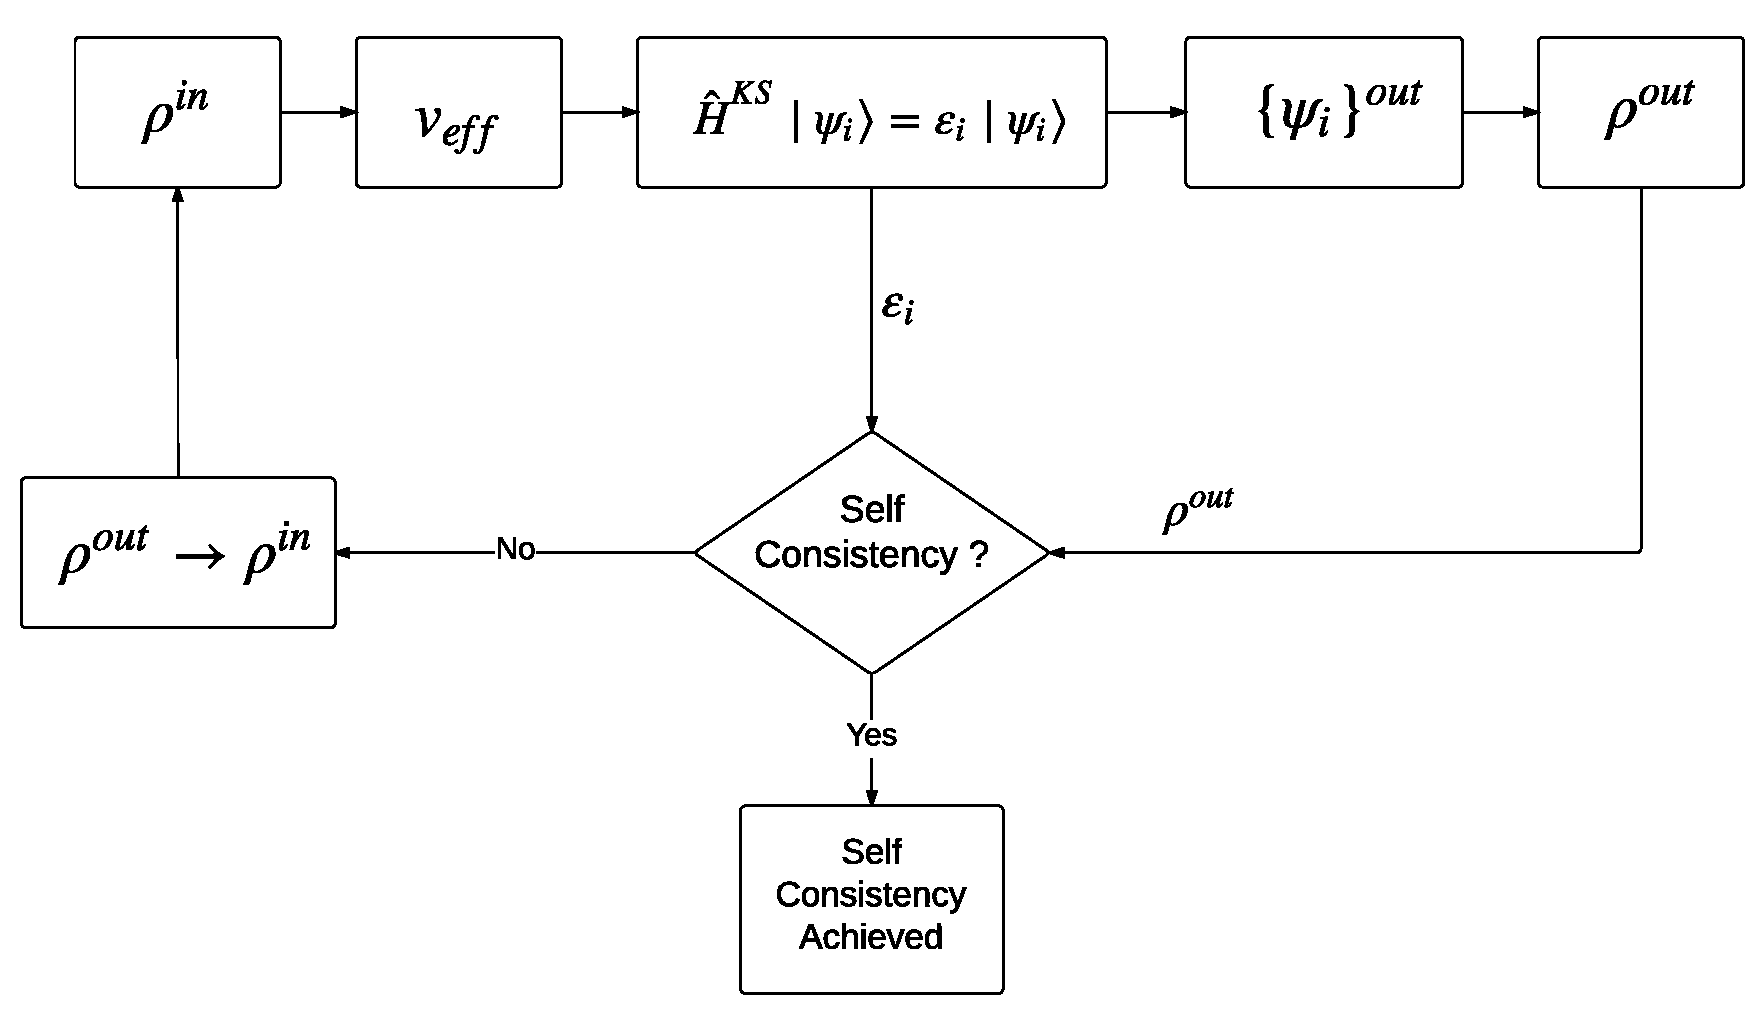
\includegraphics[width=\linewidth]{SCF-DFT_schema.pdf}	
	\end{framed}
	\caption{DFT SCF procedure layout}
	\label{fig:SCF-DFT}
\end{figure}



As one can imagine, the main computational complexity is contained in step \ref{en:SCFDiag}.
The choice of the basis set has great impact on the implementation of this procedure, both for the evaluation of $H \ket{\psi}$ and the diagonalization strategy. 

As a final consideration of this section we must say that the Kohn-Sham eigenvalues $\varepsilon^{KS}_j$ don't posses a physical meaning \cite[p.144]{Martin}, they cannot be associated with \textit{real} energies \footnote{With the exception of the highest $\varepsilon_{i}$ \cite[p.144]{Martin}}. 
The same can be said about the spatial orbitals  $\{\psi^{ks}_j\}$, which are not \textit{real} electronic orbitals. 
Nevertheless they constitute a set of useful tools to build other meaningful physical quantities, first and foremost the electronic density $\dens$.

\subsection{Lattice Structures}
It is convenient to introduce the concept of \textit{Bravais lattice} and \textit{reciprocal lattice} for their central role in solid state physics. 


\subsubsection{Bravais Lattice}
The \textit{Bravais lattice} is a set of points in real space that can be identified by the following relation :
\begin{equation}\label{eq:BravaisLattice}
	\mathbf{R} = n_{1} \mathbf{a}_{1} + n_{2} \mathbf{a}_{2} + n_{3} \mathbf{a}_{3} ,
\end{equation}
where $\{\mathbf{a}_{i}\}$ is as a set of linear independent vectors called the \textit{primitive vectors} and $n_{i}$ is always an integer number.
The definition appears clear looking at figure \ref{fig:BravaisLattice}.

\begin{figure}[h]
\begin{center}
	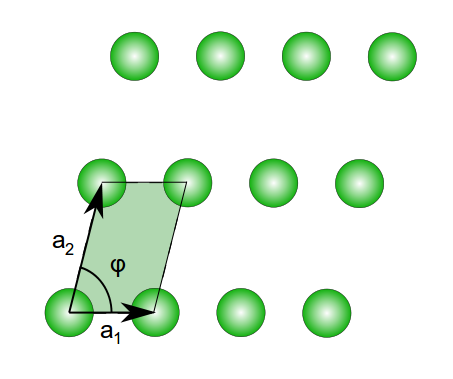
\includegraphics[width=0.4\linewidth]{Bravais_2D.png}
	\caption{Bi-dimensional Bravais lattice, with two of the possible primitive vectors.}
	\label{fig:BravaisLattice}
\end{center}
\end{figure}

Forming a matrix from the primitive vectors, one can express the volume of the primitive cell as 
\begin{align}
	\Omega = det(\left[\mf{a}_1 \mf{a}_2 \mf{a}_3\right]).
\end{align}

\subsubsection{Primitive Cell}
The \textit{primitive cell} is the single smallest portion of lattice that can generate the whole lattice by applying translation and symmetry operations.

\subsubsection{Wigner-Seitz Cell}

The \textit{Wigner-Seitz} cell around a lattice point $\mathbf{R}$ is defined as the locus of points in space that are closer to that lattice point than to any of the other lattice points (see figure \ref{fig:WSCell}).

\begin{figure}[h]
\begin{center}
	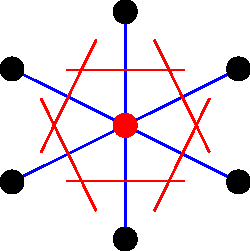
\includegraphics[width=0.4\linewidth]{Wigner.pdf}
	\caption{Bi-dimensional Wigner-Seitz cell}
	\label{fig:WSCell}
\end{center}
\end{figure}

\subsubsection{The Reciprocal Lattice}
Considering a set of $\mathbf{R}$ points constituting a Bravais lattice and a plane wave $\psi(\erre) = e^{i\mathbf{k}\cdot\mathbf{r}}$, for a generic $\mathbf{k} \in \mathbb{R}$ the plane wave $\psi(\erre)$ will be periodic on the lattice only for certain values of $\mathbf{k}$.


We call the ``\textit{reciprocal lattice}" the set $\{\mathbf{K}\}$ of points $\mathbf{k}$ for which the associated plane wave $\psi(\erre)$ is periodic in the Bravais lattice.

One can show \cite{Martin} that the reciprocal lattice is a Bravais lattice and that the following relationship (in matrix form) between the reciprocal primitive vectors $\{\mathbf{b}_i\}$ and the original primitive vectors $\{\mathbf{a}_i\}$ held:
\begin{equation}
\left[\mathbf{b_{1}b_{2}b_{3}}\right]^{T} = (2\pi^3) \left[\mathbf{a_{1}a_{2}a_{3}}\right]^{-1}
.
\end{equation}

A generic point in the reciprocal lattice is identified by the $\mathbf{G}$ vector 
\begin{equation}
	\mathbf{G} = m_1\mathbf{b_1} + m_2\mathbf{b_2} + m_3\mathbf{b_3},
\end{equation}
where $m_i$ is an integer.

Given the periodic condition, every plane wave must satisfy 
\begin{equation}
	e^{i \mathbf{G}\cdot (\mathbf{r} + \mathbf{R})} =  	e^{i \mathbf{G}\cdot \mathbf{r}},
\end{equation}
hence 
\begin{equation}
	e^{i \mathbf{G}\cdot \mathbf{R}} =  	1,
\end{equation}
equivalently 
\begin{align}
	&\mathbf{G}\cdot \mathbf{R} = 2\pi N &N\in\mathbb{Z},
\end{align}
for every $\mathbf{R}$ in the Bravais lattice.

Usually the original Bravais lattice $\{ \mathbf{R} \}$ is called the ``\textit{direct}" lattice.

Finally, the Wigner-Seitz cell of the reciprocal lattice is called the ``\textit{first Brillouin zone}".

As explained in \cite[p.121]{Manini} the reciprocal lattice is the (discrete) Fourier transform of the direct lattice.

We will see that the duality between the direct lattice and the reciprocal lattice is one of the greatest computational strength of theories based on plane waves basis sets.

\subsection{Electrons in Lattice}\label{sec:elLattice}

Solid state physics studies the properties of matter when arranged in crystal lattice form, i.e. each lattice point (or node) accommodate an atom or a molecular structure. 
Elementary cells composed by a group of nodes are then replicated trough translation and symmetry operations to generate the whole crystal.
\subsubsection{The Bloch Theorem}
Since, as we have seen before, the potential the electrons are subjected to is mainly defined by ions' positions\footnote{Remember that the Born-Oppenheimer approximations stands firmly.}, in a lattice we must expect a periodic $v_{eff}$ potential.

Namely, we have that in equation \eqref{eq:KSeq} 
\begin{equation}
	v_{eff}(\erre) = 	v_{eff}(\erre + \mf{R}).
\end{equation}
But what are the implications of this condition on the solutions of \eqref{eq:KSeq}?

The well celebrated \textit{Bloch's theorem} \cite[p.136]{Manini} answers the question.

\begin{center}
\begin{framed}

\textit{All Schr\"odinger eigenstates in a periodic potential $v_{eff}(\erre) = 	v_{eff}(\erre + \mf{R})$ can be chosen in the factorized form:}
\begin{equation}\label{eq:Bloch}
		\psi_{j}(\erre) = e^{i \mf{k} \cdot \erre } ~ u_{\mf{k}j}(\erre), 
\end{equation}
\textit{where the function $u_{\mf{k}j}(\erre)$ has the same periodicity of the lattice $u_{\mf{k}j}(\erre) = u_{\mf{k}j}(\erre + \mf{R}) $, and $\mf{k}$ is a suitable wave vector (depending on $\psi_j$, but otherwise subject to no restriction).}
\end{framed}
\end{center}

Which implies two equivalent considerations.
\begin{itemize}
	\item In a periodic context all electronic eigenfunctions have non-trivial spatial  dependence only within one primitive unit cell: in any other cell the wave function is equal to that in the original cell, apart from a constant phase factor $e^{i \mf{k} \cdot \mf{R}}$ (which leaves the probability distribution unaffected).
	\item In a periodic potential, the Schr\"odinger eigenstates are essentially plane-wave-like states, except for a periodic amplitude modulation.
\end{itemize}

If we substitute \eqref{eq:Bloch} in the Kone-Sham equations \eqref{eq:KSeq} we obtain \cite[p.137]{Manini}
\begin{framed}
\begin{equation}\label{eq:BlochEq}
	\left\lbrace -\frac{1}{2}  \left( \nabla + i\mf{k} \right)^2 + v_{eff}(\erre) \right\rbrace u_{\mf{k}j}(\erre) = \varepsilon_{\mf{k}j}  u_{\mf{k}j}(\erre),
\end{equation}
\end{framed}
which is the basic equation for stationary states of an electron characterized by a given $\mf{k}$.\footnote{Note that this result is the same for every ``\textit{mean field}" approximation (i.e. HF equations)}

The consequence of the Bloch's theorem is that, thanks to the periodicity of $u_{\mf{k}j}(\erre)$, equation \eqref{eq:BlochEq} must be solved within a single cell of the direct lattice\footnote{With applied boundaries conditions}.
This is to be compared with the solution of equations \eqref{eq:KSeq} that must be solved in the \textit{whole} crystal lattice.

Once $u_{\mf{k}j}(\erre)$ is found, the true electronic wave function $\psi_j(\erre)$ is extended to the whole lattice trough \eqref{eq:Bloch}.

Apart for the $\mf{k}$ shift of wave vector, equation \eqref{eq:BlochEq} is equivalent to a stationary Schr\"oendiger equation. Then, for a fixed $\mf{k}$, its solutions must be qualitatively similar to those of standard Schr\"oendiger equations in a finite volume, namely : a ladder of discrete eigenenergies $\varepsilon_{\mf{k}j}$ associated with eigenfunctions $u_{\mf{k}j}(\erre)$ with larger and larger number of nodes for increasing energies, labeled precisely by the index $j$.\footnote{With a noticeable parallelism to atomic orbitals.}

It is absolutely fundamental to note that $\mf{k}$ can vary freely within the first Brillouin zone; 
then for a fixed $j$ the eigenenergies $\varepsilon_{\mf{k}j}$ depends on $\mf{k}$ as \textbf{continuous} functions!

These function are called ``\textit{energy bands}" or simply ``\textit{bands}", because they varies with $\mf{k}$ within a certain energy interval. 
In general, in solids, bands of contiguous $j$ can either overlap or not; 
thus the main consequence of the Bloch's theorem is that the allowed energies forms a spectrum of bands, separated by ranges of forbidden energies (\textit{band gaps}).

\subsubsection{Plane Waves}
In a crystals, electrons are characterized by an energy spectrum somewhat intermediate between that of a free particle (plane waves with all positive energies) and that of an atom (isolated eigenvalues separated by gaps).

One possible approach to model this kind of behavior is to use plane waves as basis set for the expansion of $\psi_{j}$.
\begin{equation}\label{eq:PWExpansion}
	\ket{\psi_j}  = \sum_{\mf{k}'} c_{j\mf{k}'} \ket{\mf{k}'},
\end{equation}
where $\{\ket{\mf{k}'}\}$ is a set of ortho-normalized plane wave states $\mathbf{k'}(\erre) = \sqrt{V}^{-1} e^{i\mf{k'}\cdot\erre}$ and $c_{j\mf{k}'}$ are the Fourier expansion coefficients.\footnote{Note that in general the sum extends over all possible $\mf{k}'$, leading to an integration:
\begin{equation}
	\psi_j(\erre) = \int \varphi_j(\mf{k}) e^{i\mf{k} \cdot \erre} \dd{\mf{k}}.
\end{equation}
}

Replacing \eqref{eq:PWExpansion} in \eqref{eq:KSeq} and multiplying on the left for $\bra{\mf{k}}$ we obtain \cite{Martin} 
\begin{align}
	\bra{\mf{k}} -\frac{1}{2}\nabla^2 + v_{eff} \ket{\psi_j} &= \varepsilon_j \bra{\mf{k}}\ket{\psi_j},  \\
	\sum_{\mf{k'}} \left( \frac{1}{2}\mid\mf{k}\mid^2  \delta_{\mf{k},\mf{k'}} + \bra{\mf{k}}v_{eff}\ket{\mf{k'}} \right) c_{\mathbf{jk'}} &= \varepsilon_j \sum_{\mf{k'}} \delta_{\mf{k},\mf{k'}} c_{\mathbf{jk'}} \label{eq:SCHFourier},
\end{align}

where we have used $\bra{\mf{k}}\ket{\mf{k'}} = \delta_{\mf{k},\mf{k'}}$ and the fact that $\ket{\mf{k}}$ are eigenstates of the momentum operator.

This is the form equation \eqref{eq:DFTMatrix} takes when plane waves are used as basis set, where $\mathbf{S}$ is diagonal and $\mathbf{C}$ is composed by Fourier expansion coefficients.

Expliciting the matrix element $\bra{\mf{k}} v_{eff} \ket{\mf{k'}}$ we have \cite{Martin} 
\begin{equation}
	\bra{\mf{k}} v_{eff} \ket{\mf{k'}} = \mathcal{N} \int e^{i\left(\mf{k} - \mf{k'} \right) \cdot \erre} v_{eff}(\erre) \dd{\erre} = \tilde{v}_{eff}(\mf{k} - \mf{k'}),
\end{equation}

that are the Fourier components of the potential $v_{eff}$, where $\mathcal{N}$ is the appropriate normalizing constant.

So far we said nothing about the nature of our system, in fact equation \eqref{eq:SCHFourier} is the equivalent formulation of \eqref{eq:KSeq} in Fourier space, where in general $\mf{k}$ are continuous quantities.
This means that by using plane waves we can perform a set of calculations in the reciprocal space, and then transpose the results in the direct space trough inverse Fourier transformations.

If we introduce the condition of a periodic potential, as a consequence of the Bloch's theorem, we have that $\tilde{v}_{eff}(\mf{k} - \mf{k'})$ is not-null only when $\mf{k} - \mf{k'} = \mf{G}$, where $\mf{G}$ is a vector of the reciprocal lattice \cite{Martin}.

This means that in the continuous-indexed energy matrix of eq \eqref{eq:SCHFourier} most off-diagonal elements vanishes because for the element to be not-null the following relation must stand $\mf{k} = \mf{k'} + \mf{G}$.

Then the continuous-indexed $\mf{H}^{KS}$ matrix becomes a diagonal discrete-indexed block matrix, meaning that one can diagonalize only the non-null blocks on the diagonal, and, more importantly, the operation can be performed independently for each block (i.e. in parallel!).

For computational purposes the discrete index is obviously a great advantage, but we still have to address the problem that we need an infinite number of $G$ to completely describe the system.
Following the same process of the Hartree-Fock method, we select only a subset of all the possible plane waves by imposing a condition on the energy of the plane wave, the so-called \textit{cutoff energy}:
\begin{align}
	\mf{k'}(\erre) = e^{i(\mf{k + G}) \cdot \erre};\\
	\frac{\hbar^2}{2m_e}\mid \mf{k + G} \mid < E_{cut}. \label{eq:cutoffEnergy}
\end{align}

In order to pick the correct cutoff energy a series of tests can be performed beforehand with little (and constant) computational effort.

We can now summarize the advantages of plane waves basis sets in periodic potentials:
\begin{enumerate}
	\item It is possible to perform calculations in the reciprocal space and then transpose the result in the direct space. Remember that differentiating in direct space corresponds multiplication in reciprocal space! This greatly simplify the calculation on kinetic terms, and often also of $E_{xc}$.\footnote{As said before, the functional is often expressed in function of $(\dens,\grad\dens,\nabla^2\dens)$.}
	\item The continuous indexed matrix $\mf{H}^{KS}$ becomes a finite discrete-indexed matrix.
	\item The $\mf{H}^{KS}$ matrix becomes diagonal at blocks, and each block can be diagonalized in parallel. \label{en:Kpoints}
\end{enumerate}

Point \ref{en:Kpoints} is the so-called \textit{K-points parallelization}, and, as one can image, it has a great impact on the resolution of the electronic problem in symmetric crystals.

In this work we mainly focused on the study of systems having little symmetries\footnote{Non-periodic systems usually has peculiar physical properties, this is why they are of great research interest and why we focused on them.}, this implies the enlargement of the elementary cell to accommodate all asymmetric factors. 
As a result the $\mf{H}^{KS}$ matrix becomes occupied mostly by a single block and no k-points parallelization can be performed.
This configuration is usually referred as \textit{Gamma point}.



\subsubsection{Grid representation and the size of the problem} \label{sec:Grid}

Thanks to the Bloch's theorem, the calculation for each $\mf{k}$ point is independent and, as said above, we focused on systems in gamma-point configuration. 
%then for the sake of simplicity we will consider $\mf{k}=0$.

Consequently, any of the following considerations is valid within a given (and fixed) k-point sub-block of $\mf{H}^{KS}$.

We know that the solutions to equation \eqref{eq:BlochEq} are in factorized form :
\begin{align}
	\psi_{j}(\erre,\mf{k}) &= e^{i \mf{k} \cdot	 \erre} u_{\mf{k},j}(\erre,\mf{k}), \\
	u_{\mf{k},j}(\erre,\mf{k}) &= \frac{1}{\sqrt{\Omega}} \sum_{\GI} c_{j}(\GI,\mf{k})e^{i \GI \cdot \erre}.
\end{align}

Using the above convention $u_{\mf{k},j}(\erre,\mf{k})$ became:

\begin{align}
	u_{kj}(\erre) = \frac{1}{\sqrt{\Omega}} \sum_{\GI} c_{kj}(\GI)e^{i \GI \cdot \erre},
\end{align}

being $c_{kj}(\GI)$ the Fourier expansion coefficients, it coincides with a discrete Fourier transformation.

The expansion is truncated using equation \eqref{eq:cutoffEnergy} to a certain $\mid \GI \mid < G_{cut}$ (where $G_{cut}$ is the maximum module of a reciprocal vector below the cutoff energy \eqref{eq:cutoffEnergy}), fixing the size of the basis set. This can be done because $v_{eff}$ converge rapidly with increasing modulus of $\GI$.

According to \cite[p.88]{Marx} a rough estimate of the number of plane waves is \footnote{With both $\Omega$ and $E_{cut}$ expressed in atomic units.}
\begin{equation}\label{eq:NGPW}
	N_{G}^{PW} = \frac{1}{2\pi^2}\Omega E_{cut}^{\frac{3}{2}}.
\end{equation}

A function given as a finite linear combination of plane waves can also be defined as a set of functional values on an equally spaced grid in real space.

The sampling theorem gives the maximal grid spacing
that still allows us to hold the same information as the expansion coefficients
of the plane waves. The real space sampling points $\mf{R}$ are defined as: 

\begin{equation}
	\mf{R} = \left[\mf{a}_1 \mf{a}_2 \mf{a}_3 \right] \mf{N} \mf{q},
\end{equation}

where N is a diagonal matrix with the entries $1/N_i$, $\mf{q}$ is a vector of
integers ranging from $0$ to $N_i - 1$ and $i = x, y, z$. 

In order to fulfill the
sampling theorem $N_i$ has to be bigger than $2 max(\mf{b}_i) + 1$\footnote{Where $\mf{b}_i$ is a primitive vector of the reciprocal lattice}. 
In addition, $N_i$ must be decomposable into small prime numbers (typically 2, 3, and 5) when fast Fourier transformation techniques are used.
In practice, the smallest number $N_i$ that fulfills the above requirements is
chosen.

A periodic function can be calculated at the real space grid points $\mf{R}$ as \cite[p.89]{Marx} :
\begin{align}
	f(\erre) &= \sum_{\GI} \tilde{f}(\GI) e^{i \GI \cdot \erre} \\
			 &= \sum_{\mf{b}} \tilde{f}(\GI) exp\left[ \frac{2\pi}{N_{x}} i b_x q_x \right]  exp\left[ \frac{2\pi}{N_{y}} i b_y q_y \right]  exp\left[ \frac{2\pi}{N_{z}} i b_z q_z \right], \label{eq:FFTDef}
\end{align}
where we have expanded every $\GI$ in a linear combination of the primitive reciprocal vectors $\{\mf{b}_i\}$.

The function $\tilde{f}(\GI)$ is zero outside the cutoff region, and the sum over the \textbf{b}-vectors can be extended over all indices in the cube $-\mf{b}_{i}^{max} , \cdots ,\mf{b}_{i}^{max}$ . 

The functions $f(\mf{R})$ and $\tilde{f}(\GI)$ are related
\begin{align}
	f(\mf{R}) &= IFT[ \tilde{f}(\GI) ]\\
	\tilde{f}(\GI) &= FT[ f(\mf{R}) ].
\end{align}

The calculation of the three-dimensional Fourier transforms can be performed by a
series of one-dimensional Fourier transforms \cite{Marx}. The number of transforms in
each direction is $N_y N_z$ , $N_x N_z$ , and $N_x N_y$ , respectively. Assuming that the
one-dimensional transforms are performed within the fast Fourier transform
framework, the number of operations per transform of length $n$ is approximately $\mathcal{O}(n log(n))$. This leads to an estimate for the number of operations for the full three-dimensional transform of $\mathcal{O}(N log(N))$ , where $N = N_x N_y N_z$ .

Because to use the FFT a regular grid in the form of a parallelepiped is needed (both in direct and reciprocal space), the number of points in the FFT grid for density $N = N_{R} = N_{G}$ is roughly an order of magnitude larger than the number $N_{G}^{PW}$ defined in \eqref{eq:NGPW} \cite{Martin}.

See table \ref{tab:FFTSummary} for a summary of the relationships between direct and reciprocal grid and an estimate of their typical dimensions.

\begin{table}[]
\centering
\begin{tabular}{lc}
\hline
\multicolumn{1}{|l|}{\textbf{Size}} & \multicolumn{1}{l|}{\textbf{Description}}                                                                                                                        \\ \hline
\multicolumn{1}{|l|}{$N_{R}$}       & \multicolumn{1}{l|}{Number of $\mf{R}$ points in the real grid}                                                                                                  \\ \hline
\multicolumn{1}{|l|}{$N_{G}$}       & \multicolumn{1}{l|}{Number of $\GI$ points in the reciprocal grid}                                                                                               \\ \hline
\multicolumn{1}{|l|}{$N_{G}^{PW}$}  & \multicolumn{1}{l|}{\begin{tabular}[c]{@{}l@{}}Number of $\GI$ points in the reciprocal grid associated to \\ plane waves below the cutting energy\end{tabular}} \\ \hline

                                    & \multicolumn{1}{l}{}                                                                                                                                             \\ \cline{2-2} 
\multicolumn{1}{l|}{}               & \multicolumn{1}{c|}{\textbf{Relationships}}                                                                                                                      \\ \cline{2-2} 
\multicolumn{1}{l|}{}               & \multicolumn{1}{c|}{$N_{R} = N_{G} = N = N_x N_y N_z$}                                                                                                                         \\ \cline{2-2} 
\multicolumn{1}{l|}{}               & \multicolumn{1}{c|}{$N_{G}^{PW} < N$}                                                                                                                       \\ \cline{2-2} 
\multicolumn{1}{l|}{}               & \multicolumn{1}{c|}{\textbf{Estimate for a 100 atom system}}                                                                                                                       \\ \cline{2-2} 
\multicolumn{1}{l|}{}               & \multicolumn{1}{c|}{ $N_{b} \simeq \frac{1}{2} N_{e^{-}} \simeq 10^3~;~ N_{G}^{PW} \simeq 10^{6} ~;~ N \simeq 10^7 $}                                                                                                                       \\ \cline{2-2} 
                                    &                                                                                                                                                                  \\ \cline{2-2} 
\multicolumn{1}{l|}{}               & \multicolumn{1}{c|}{\textbf{Computational cost of every Fast Fourier Transform}}                                                                                           \\ \cline{2-2} 
\multicolumn{1}{l|}{}               & \multicolumn{1}{c|}{$\mathcal{O}(N log (N))$}                                                                                                                    \\ \cline{2-2} 
\end{tabular}
\caption{Summary of typical dimensions between direct and reciprocal grid}
\label{tab:FFTSummary}
\end{table}



We shall now proceed with an in-depth analysis of the implementation of DFT SCF methods in the Quantum ESPRESSO suite, one of the most popular and solid software for materials modeling.


\newpage

%----------------------------------------------------------------------------
\section{\QE}\label{sec:QE}
%----------------------------------------------------------------------------

\QE  is an integrated suite of computer codes for electronic-structure calculations and materials modeling based on density-functional theory, plane waves basis sets and pseudopotentials to represent electron-ion interactions.

\QE is free, open-source software distributed under the terms of the GNU General Public License (GPL) and is written, mostly,in Fortran-95, with some parts in C or in Fortran-77.

\QE core features are implemented leveraging the well optimized versions of linear algebra and parallelization libraries like BLAS, LAPACK, SCALAPACK, FFTW, that are easily available for a wide range of computational architectures.

The MPI standard\cite{MPI} is used for interprocess communication and the OpenMP standard\cite{OMP} is used for thread parallelization.


\QE has been compiled and tested on numerous computing systems\cite{QEManual}: i386 Linux desktops, i386 Linux clusters, Mac OS X, Cray machines, IMB AIX, IBM BlueGene, NUMA machines, Intel-Phi co-processors, CUDA accelerators, FPGA accelerators and even mobile devices. 

Quantum ESPRESSO distribution is composed by a set of packages (executables) built upon a versatile core library, a complete list of executables and various features can be found in \cite{QE}.

In our work we focused only on the \textit{PWscf} package, which implements an iterative approach to reach self-consistency, using at each step iterative diagonalization techniques, in the framework of plane waves basis set.


\subsection{SCF Implementation in \textit{PWscf} package}
In section \ref{sec:SCF-DFT} we gave a basic representation of an SCF algorithm based on DFT.

In section \ref{sec:elLattice} we saw how the choice of plane waves as basis set impacts on the solution of Kohn-Sham equations.

Finally, in section \ref{sec:Grid} we showed how direct and reciprocal space are represented and how it's possible to move from one representation to another. 
\QE leverages this feature to calculate the terms in $\mf{H}^{KS}$ where it is more convenient to.


In the following section we will show the calculations needed to perform each SCF step as implemented in PWscf package.

As a reference, we will use  the steps outlined in figure \ref{fig:SCF-DFT} on page \pageref{fig:SCF-DFT}.
The figure is reprinted here to help the reader.

\begin{figure}[h]
\begin{center}
	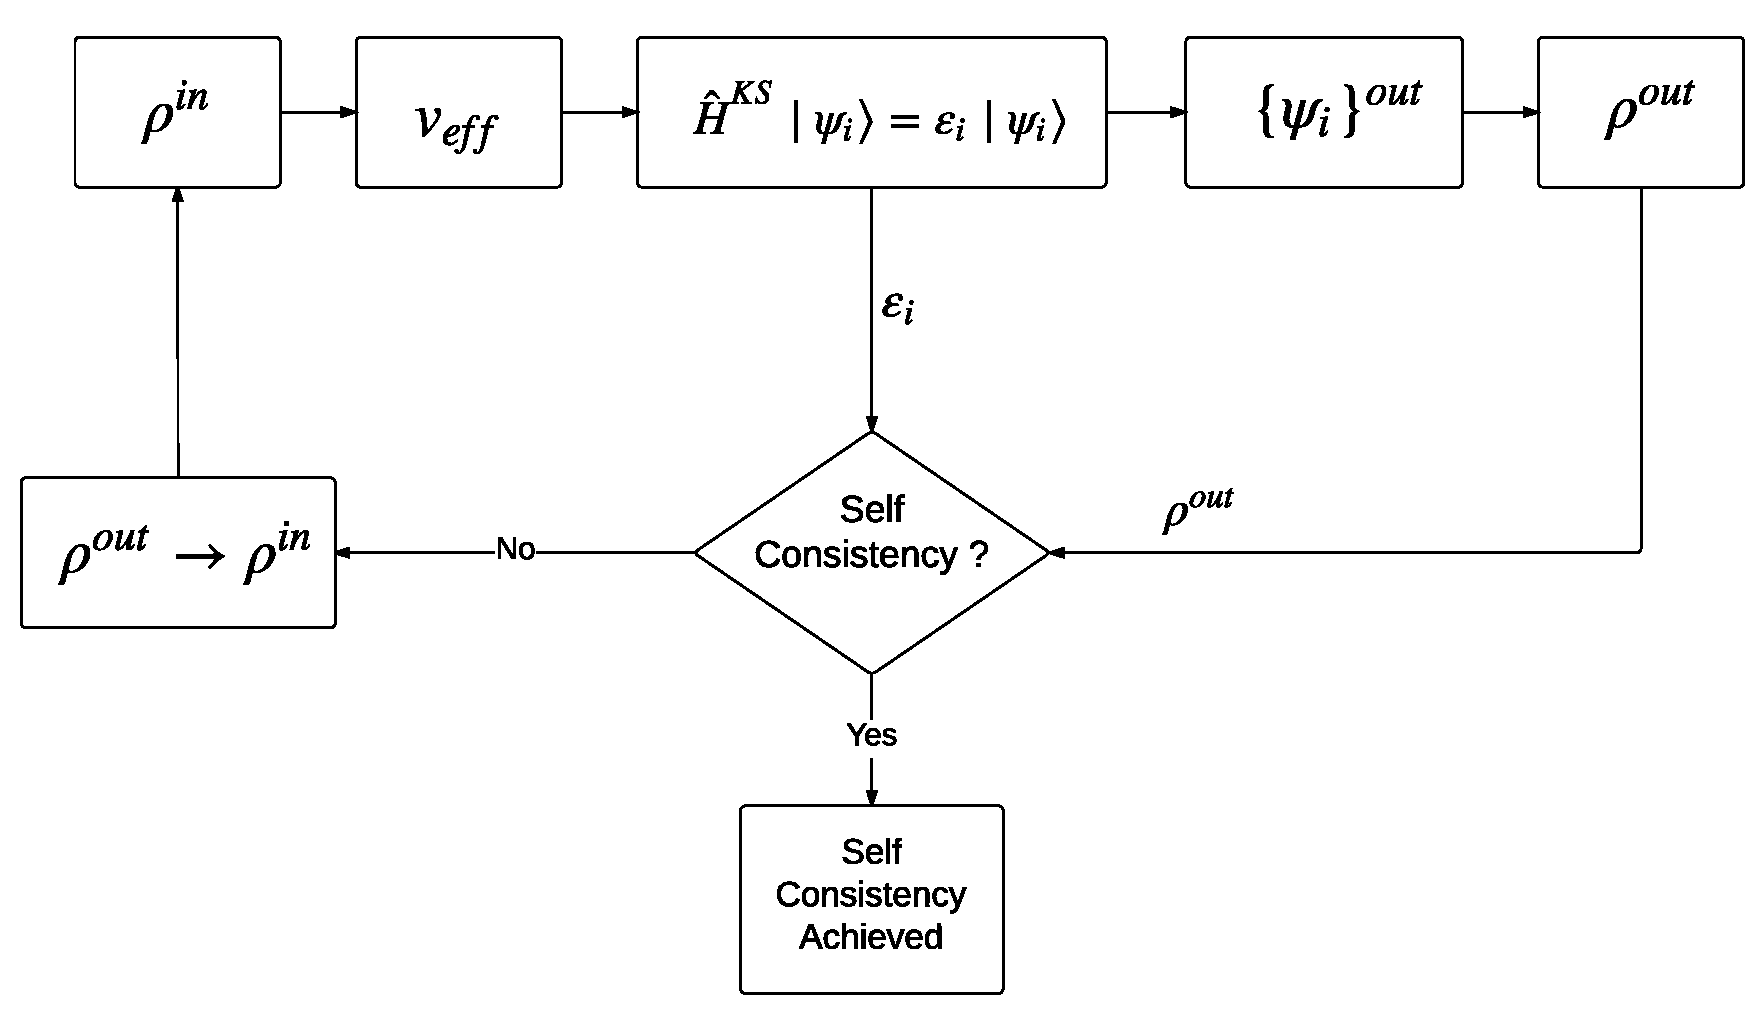
\includegraphics[width=\linewidth]{SCF-DFT_schema.pdf}	
	\end{center}
\end{figure}

\subsection{Initialization (Step 0)}
For the SCF iteration to be performed, a set of preliminary initializations must occur.
This preliminary step is implemented within the \texttt{init\_run} subroutine.

Besides the allocation of all the buffers and the tuning of grid dimensions\footnote{Remember that for the FFT to perform well, the number of points per dimension must be a multiple of a prime number, see sec \ref{sec:Grid}}, the real goal of this step is to obtain an initial electronic density $\dens$ and an estimate of the total energy of the system.

As a default behavior, \QE combines the electronic densities of every atomic species within the elementary cell.
The same is done for the atomic orbitals, composing a preliminary set of Kohn-Sham orbitals $\{\psi_j\}$.
\footnote{This is the default behavior of \QE ,it is also possible to perform a random initialization.}

Using $\dens$ to evaluate $v_{eff}$ and $\{\psi_j\}$ to compute $\mf{H}_{ij}^{KS}$, $\mf{H}^{KS}$ is diagonalized to obtain the initial energy of the system thanks to equation \eqref{eq:DFTEnergy}. 

The results of this preliminary step will be used as a starting point in points one, two and four of figure \ref{fig:SCF-DFT}.

Note that this first diagonalization is much faster than the ones performed during the SCF iteration.




\subsubsection{Evaluating the potential (Step 1)}\label{sec:Potential}

The potential $v_{eff}$ is composed by three terms:
\begin{equation}
	v_{eff} = v + v_{h} + v_{xc},
\end{equation}
where $v$ is the electron-ion potential, $v_{h}$ the electrostatic Hartee potential and $v_{xc}$ is the exchange-correlation potential\footnote{The ``spatial" dependency of the potentials will be explicited when needed.}.

\paragraph{The electron-ion potential:}
$v$ was originally defined in \eqref{eq:electronionPotential} considering every ion as a point-like distribution of charge. 
However, since we choose plane waves as basis set, modeling the behavior of electrons in the valence band (strongly localized around each ion) is rather difficult due to the delocalized nature of plane waves.

Nevertheless plane waves suit greatly the description of electrons in the conduction bands: since the ionic potential they are subject to is screened by valence electrons\cite[p.136]{Manini}, they result more delocalized, especially in lattice crystals.

To model this dual nature without having to enlarge wildly the basis set to describe valence electrons\footnote{i.e. using an high number of Fourier coefficients in \eqref{eq:PWExpansion}, hence a large cutoff energy.}, \QE uses the so-called \textit{pseudopotentials} theory.

A discussion on the nature of pseudopotentials is out of the scope of this work, however a good dissertation on the matter can be found in \cite[chap. 11]{Martin} and \cite[p.90]{Marx}.
What we need to know about pseudopotentials is that the electron-ion potential generated by a single ion can be expressed in reciprocal space as :
\begin{equation}
	\tilde{v}_{\alpha}(\mf{G}) = \sum_{\mf{G}} f_{ps}^{sp}(G) e^{i \mf{G} \cdot \mf{R}_{\alpha}},
\end{equation}
where  $\mf{R}_{\alpha}$ is the position of the ion and $f_{sp}^{sp}(G)$ is the function describing the pseudopotential of the given atomic species ``\textit{sp}" (e.g. hydrogen, oxygen, sodium, ...).

Given the position of each ion within the elementary cell and its atomic species, $\tilde{v}(\mf{G})$ is calculated as a superposition of each $\tilde{v}_{\alpha}(\mf{G})$.

Note that because ions' position is fixed under the Born-Oppenheimer approximation, $\tilde{v}(\mf{G})$ is calculated only once for the whole SCF iteration, then its impact on the computational cost is negligible.  

As said above, the calculation of $\tilde{v}(\GI)$ happens inside the \texttt{init\_run} routine in the first evaluation of $v_{eff}$.

\mynotes{in realta' puo' essere costoso anche applicarli gli pseudopotenziali per via di come sono fatti. (Davide)}

\paragraph{The Hartree Potential:}

$v_{h}(\erre)$ is defined in \eqref{eq:HartreePot} as 
\begin{equation}
 v_{h}(\erre) = \int \frac{\rho(\mathbf{r'})}{\mid \mathbf{r} - \mathbf{r'} \mid}  \dd{\mathbf{r'}}.
\end{equation}

$v_{h}$ is nothing else than the classical electrostatic potential generated by a tridimensional distribution of charge with volumetric charge density $\rho(\erre')$.

We know that every electrostatic potential must satisfy the Poisson's equation :
\begin{equation}\label{eq:Poisson}
	\nabla^2 v_{h}(\erre) = - \frac{\dens}{\varepsilon_{0}},
\end{equation} 
where $\varepsilon_{0}$ is the dielectric constant $(4\pi e^2)^{-1}$.

Equation \eqref{eq:Poisson} in reciprocal space becomes:
\begin{equation}\label{eq:HartreePotReciprocal}
	\tilde{v}_{h}(\mf{G}) = \frac{\tilde{\rho}(\mf{G})}{G^2 \varepsilon_{0}},
\end{equation}
where $\tilde{v}_{h}(\mf{G})$ and $\tilde{\rho}(\mf{G})$ are the Fourier transforms respectively of $v_{h}(\erre)$ and $\dens$.

Instead of having to compute the integral in \eqref{eq:HartreePot}, we just need the expression of $\tilde{\rho}(\mf{G})$.
This is undoubtedly a great advantage from a computational standpoint, because all the complexity lies in the evaluation of $\tilde{\rho}(\mf{G})$, which is performed at the beginning of every iteration step as an FFT of $\dens$.
Hence the computational cost associated to $v_{h}$ is $\bigO(N log(N))$.

Using the definition \eqref{eq:HartreePot} would require to compute the integral for every point of the real grid . That is : for every of the $N$ point of the real grid (labeled by $\mf{r}$) one must sum (integrate) again for every point of the real grid $N$ (labeled by $\mf{r}'$). 
This would lead to a complexity of $\mathcal{O}(N^2)$.

For the sake of simplicity we can derive equation \eqref{eq:HartreePotReciprocal} in one dimension.

\begin{equation} \label{eq:PossionMono}
	\pdv[2]{v_{h}(x)}{x} = - \frac{\rho(x)}{\varepsilon_0},
\end{equation}
then 
\begin{align*}
	v_{h}(x) &= \frac{1}{\sqrt{2\pi}} \int \tilde{v}_{h}(g) e^{i g x} \dd{g}; \\
	\rho(x) &= \frac{1}{\sqrt{2\pi}} \int \tilde{\rho}(g) e^{i g x} \dd{g}.
\end{align*}

Replacing into  \eqref{eq:PossionMono} and differentiating, we obtain :
\begin{equation}
	\frac{g^2}{\sqrt{2\pi}} \int \tilde{v}_{h}(g) e^{i g x} \dd{g} = \frac{1}{\varepsilon_{0}\sqrt{2\pi}} \int \tilde{\rho}(g) e^{i g x} \dd{g},
\end{equation}
hence 
\begin{equation}
	\tilde{v}_{h}(g) = \frac{\tilde{\rho}(g)}{g^2 \varepsilon_{0}}.
\end{equation}



\paragraph{Exchange correlation potential:} 
As explained in section \ref{sec:SCF-DFT}, $E_{xc}[\dens]$ is fixed at the beginning of the SCF iteration and never changes trough the whole iteration. $v_{xc}(\erre)$ is obtained analytically trough equation \eqref{eq:ExchangePotDer}.

Even if $v_{xc}(\erre)$ is computed at the beginning of each iteration step, because $E_{xc}[\dens]$ depends on the electronic density, the computational cost of \eqref{eq:ExchangePotDer} is negligible.


~


We now have an expression for all the terms in $v_{eff}$, but two of them ($\tilde{v}_{h}$ and $\tilde{v}$) are calculated in the reciprocal space.

Since $v_{eff}$ is applied in the direct space, where it's a trivial multiplicative operator, we need to inverse transform $\tilde{v}_{h}$ and $\tilde{v}$.

We have that
\begin{equation}
	v_{eff}(\erre) = IFFT\{\tilde{v}(\mf{G})\}(\erre) + IFFT\{\tilde{v}_{h}(\mf{G})\}(\erre) + v_{ex}(\erre).
\end{equation}

This operation is performed once for every iteration step.

\subsubsection{The kinetic term}\label{sec:KineticTerm}

Another great advantage of plane waves is that differentiation against the state function becomes a mere multiplication in reciprocal space.

In fact we have that 
\begin{equation}
	\nabla^2 u_{kj}(\erre) = \sum_{\mf{G}} - c_{kj}(\mf{G})  G^2  e^{i \GI  \cdot \erre}.
\end{equation}


\subsection{Diagonalization (Step 2)}
The diagonalization of $\mf{H}^{KS}$ is the core problem of any SCF implementation.

As specified in \cite[Appendix A.2]{QE}, the strategy adopted by \QE is to use the \textit{Davidson method}\cite{Davidson}\footnote{\QE has also an alternative algorithm, called the \textit{conjugate gradient} method.}.

The Davidson method follows an iterative approach to the solution of the eigenvalue problem.
One of the great advantages of this method is that it is possible to obtain the set of the $n$ eigenvectors with the lower (or upper) eigenvalues without performing the diagonalization of the whole $\mf{H}^{KS}$ dense matrix of dimension $N_{G}^{PW} \cdot N_{G}^{PW} \simeq N^2$.

Instead, the $\mf{H}^{KS}$ matrix is reduced in a smaller matrix which generic element is 
\begin{equation}\label{eq:DavidsonMatrix}
	\mf{H}_{ij} = \bra{u_{ki}}\mf{H}^{KS}\ket{u_{kj}},
\end{equation}
where $\ket{u_{kj}}$ is a trial eigenvector. 
Then the size of the matrix is reduced to $N_{b}^2$, to be diagonalized with standard techniques implemented in \QE using LAPACK or SCALAPACK libraries.
This drastically decreases the amount of memory needed to perform the diagonalization.

From equation \eqref{eq:DavidsonMatrix} we can see that for the algorithm to work it is necessary to implement just one basic operation: the application of the matrix to a generic state vector
\footnote{The braket calculation $ \bra{u_{ki}} (\mf{H}^{KS}\ket{u_{kj}})$ is trivial using LAPACK or SCALAPACK libraries.}
\begin{equation}
	\mf{H^{KS}} \ket{u_{kj}}.
\end{equation}
In \QE this operation is implemented inside the well-named subroutine \texttt{h\_psi} and is performed in the reciprocal space (see figure \ref{fig:hpsi}).

The evaluation of $\mf{H^{KS}}$ is divided in the kinetic term $\nabla^2$ and the potential term $v_{eff}$, each term is applied sequentially; 
the trial eigenvectors $\{\ket{u_{kj}}\}^{in}$  are the ones obtained in the previous SCF step, if any, or the ones obtained from \texttt{init\_run}.
\footnote{When the SCF step has converged, the $\{\ket{u_{kj}}\}^{out}$ obtained are not subjected to mixing, unlike $\densout$. The reason is that the amount of memory needed to store them would be too much. 
As a matter of fact $\densin$ can not be generated from $\{\ket{u_{kj}}\}^{in}$.
This in not important because the Davidson method, which is iterative, will guarantee the convergence to the real $\{\ket{u_{kj}}\}^{out}$. 
$\{\ket{u_{kj}}\}^{in}$ have to be considered as a reasonable guess of the new eigenstates $\{\ket{u_{kj}}\}^{out}$, reducing the number of Davidson steps required to reach convergence.
}

As we said in section \ref{sec:KineticTerm}, the application of the kinetic term in the reciprocal space accounts just for a multiplication over $N^{PW}_G$.

In section \ref{sec:Potential} we showed that $v_{eff}(\erre)$ is calculated once per SCF iteration step, then it is fixed during the whole Davidson iteration. Since we are in the reciprocal space but $v_{eff}$ is multiplicative only in real space it is necessary to: 
\begin{enumerate}
	\item transform $\tilde{u}_{jk}(\GI)$ in $u_{kj}(\mf{R})$ using IFFT;
	\item multiply $v_{eff}(\mf{R})$ for $u_{kj}(\mf{R})$ for every $\mf{R}$ in the real grid;
	\item transform the result in reciprocal space : \\ $[v_{eff}(\mf{R}) u_{kj}(\mf{R})](\GI) = FFT\{v_{eff}(\mf{R}) u_{kj}(\mf{R})\}$;
\end{enumerate}

\begin{figure}[h]
\begin{center}
	\begin{framed}
	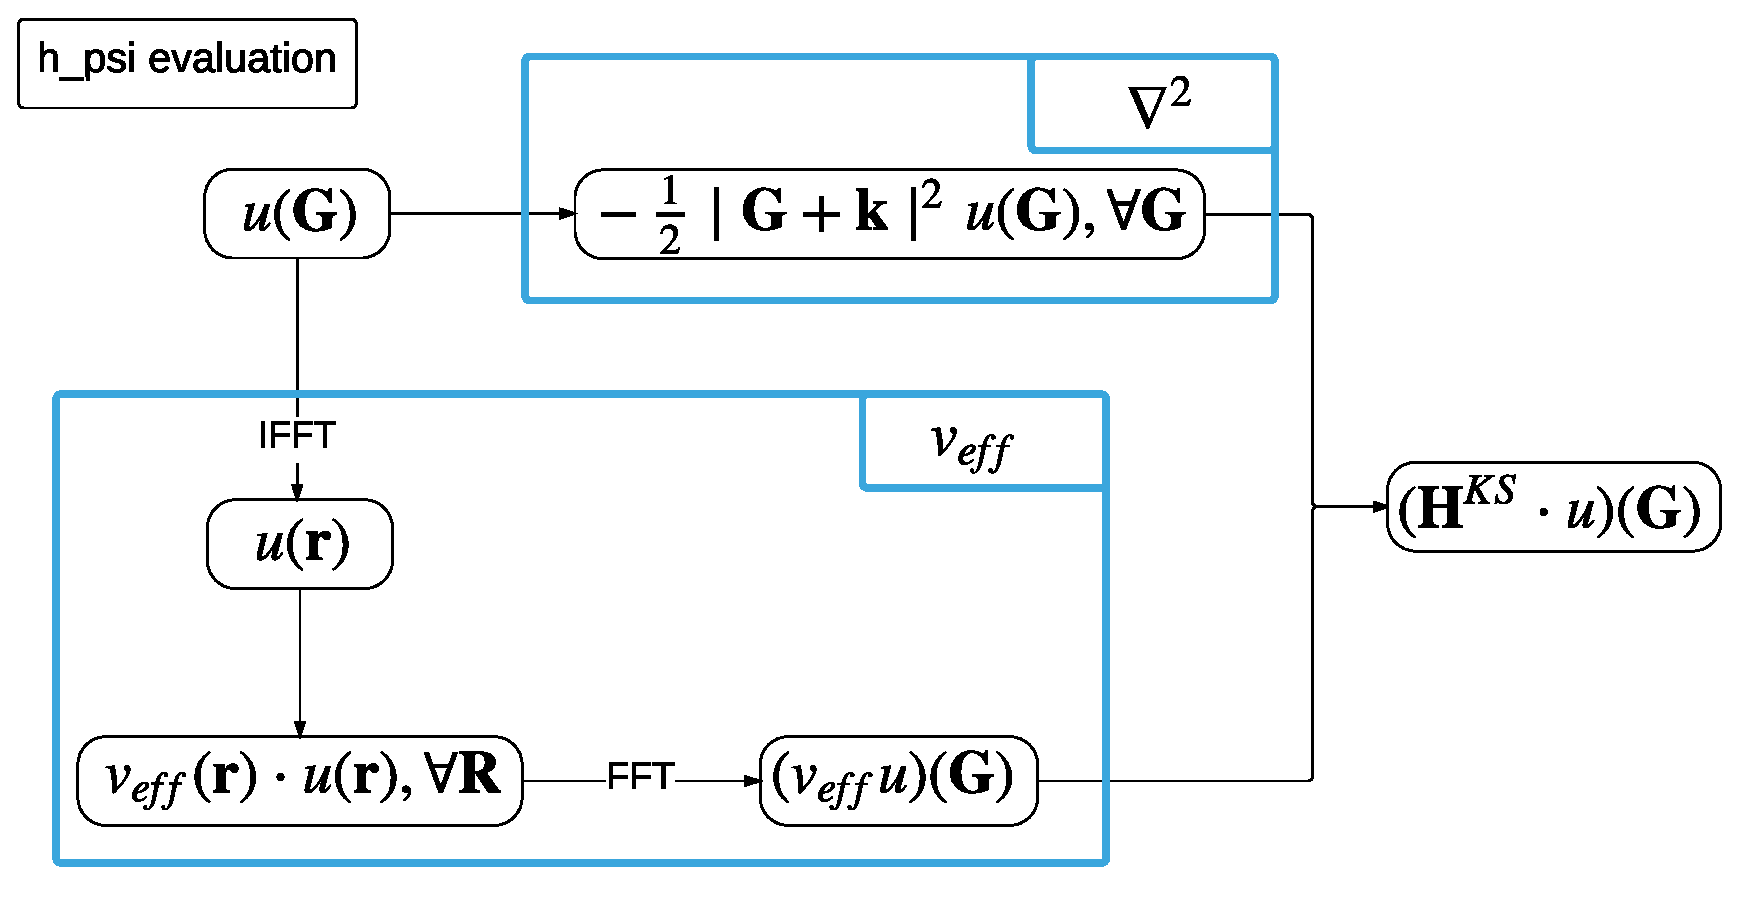
\includegraphics[width=\linewidth]{h_psi.pdf}

	\end{framed}
\caption{Implementation of \texttt{h\_psi} subroutine in \QE}
	\label{fig:hpsi}
\end{center}
\end{figure}


This means that for every call of \texttt{h\_psi} an FFT and an IFFT must be performed, each of them with complexity $\bigO(N log (N))$. 

Since \texttt{h\_psi} is called once over all the $\{u_{kj}\}$, the total complexity per iteration step is $\bigO(N_{b} N log (N))$, where $N_{b}$ is the number of bands (that is of the order of the number of electrons in the system\footnote{Neglecting spin effects, $N_b = 1/2 N_e$.}). 

Note that this is the complexity of a single Davidson iteration, the number of iterations required to solve the eigenvalue problem cannot be predicted beforehand but the computational cost of the whole Davidson diagonalization\footnote{Excluding the evaluation of $\mf{H}^{KS}$} goes as $\bigO(N_{b}^3)$ and is usually accounted as the global computational complexity of the whole DFT-SCF computation.

\subsubsection{FFT implementation}
Given their central role, it is convenient to outline how FFT transformations are performed inside \QE .
We can explicitly rewrite equation \eqref{eq:FFTDef} for an IFFT from reciprocal to real grid.

\begin{align}
	IFFT[f(\GI)] &= \sum_{j}^{N_x} \sum_{k}^{N_y} \sum_{l}^{N_z} f^{\GI}_{jkl}
		exp \left[i \frac{2\pi}{N_x}ju \right] 
		exp \left[i \frac{2\pi}{N_y}kv \right] 
		exp \left[i \frac{2\pi}{N_x}lw \right] \\
		[u,v,w] &= \mf{q} \\
		[j,k,l] &= \mf{b}_i.
\end{align}
This factorized form can be implemented as a series of three nested cycles, one for each dimension.
Usually the cycle on the $z$ axis (index $l$) is the first to be performed:
\begin{equation}\label{eq:NestedFFT2}
	IFFT[f(\GI)] = \sum_{j}^{N_x} \sum_{k}^{N_y} 
		exp \left[i \frac{2\pi}{N_x}ju \right] 
		exp \left[i \frac{2\pi}{N_y}kv \right] 
		\sum_{l}^{N_z} 	f^{\GI}_{jkl} exp \left[i \frac{2\pi}{N_x}lw \right].
\end{equation}
What \QE does is to divide the grid in a set of $N_x \cdot N_y$ columns along the $z$ axis, then the sum is performed in parallel for each column. 
This parallelization is implemented using MPI, that is : each rank calculates sequentially a set of columns.
Since the terms in the rightmost sum in \eqref{eq:NestedFFT2} are independent from one another, the sum over each column can be parallelized. 
This second layer of parallelization is performed using thread parallelization, thanks to the OpenMP library.
Being every term independent, there are no race-conditions between threads, they do not need to wait the computation performed by other threads and they work on independent chunks of memory. \footnote{See section XXX for the effects of threads overload.}

Once the sum on z columns is completed, the grid is separated in horizontal layers. 
The layers are grouped in function of the MPI ranks and bidimensionals FFT are perfomed; the second thread parallelization can still be used.

\QE uses the well known library FFTW (``Fast Fourier Transform in the West")\cite{FFTW} to perform one dimensional transformations. 
Even if a native parallel implementation of tridimensional transformations was developed in FFTWv3, \QE uses his own parallelization strategy. 
This design was developed when architectures like CrayAX an Sun HPC solutions where still supported. It was common for this kind of architectures to expose native and well optimized implementations of one-dimensional FFT transformations.

\subsubsection{Dense matrices diagonalization}

As said above, the Davidson method reduces the problem to the diagonalization of a $N_{b}^2$ matrix.
\QE can perform this operation either in parallel or serially.
The kind of parallelization used can be manually set or automatically decided.

\paragraph{Serial diagonalization: }  In this case, only one MPI rank performs the diagonalization.
\footnote{Actually, depending on the version of \QE, a set of different ranks would perform the same operation, obtaining the same result.}
Be aware that thread parallelization is still an option, if threads are enabled and the threaded version of MKL libraries have been linked.
See section XXX for an test case analysis of this scenario.

\paragraph{Parallel Diagonalization: } In this case \QE leverages the features of the SCALAPACK library and distribuite the load over a set of MPI ranks. 
Not all the ranks will be used: depending on the total number of ranks or on user setting, a number ranging from one-forth to one-half of ranks will be used. 
These ranks will be equally spaced and distributed over the whole computational resource, this is done to prevent the overload of the memory controller of a single machine.
Thread parallelization can still be performed, as noted above.
\mynotes{Se riusciamo proviamo a vedere cosa succede sulla numa se gli mettiamo i rank vicini, sulla stessa piastra. Bisogna patchare il codice.}


\subsection{Calculation of the electronic density (Step 3)}

After Davidson's diagonalization is concluded, a set $\{ u_{kj}(\GI) \}$ of $N_{b}$ eigenstates with the lowest energy is obtained.

To obtain the final density in real space it is convenient to use equation \eqref{eq:densityDef}, but, to do so, one need to transform $\{ u_{kj}(\GI) \}$ in $\{ u_{kj}(\erre) \}$ using an IFFT \cite[p.246]{Martin}.

The IFFT transform constitute the major computational cost, and it's comparable with the cost of a single Davidson step.

The procedure is implemented inside the routine \texttt{sum\_band}, which is also responsible for the computation of occupations and the sum of eigenvalues.


\subsection{Convergence criteria (Step 4)}
As explained in \ref{sec:SCF-DFT} a set of convergence test can be performed on $\densout$ and $E[\densout]$.
\QE uses a refined methods that estimates the impact of the difference between $\densout$ and $\densin$ on the energy of the system.
First we define the difference between $\densout$ and $E[\densout]$ as 
\begin{equation}
	\Delta\dens = \densin - \densout.
\end{equation}
Then we consider the terms in $E[\dens + \Delta\dens] - E[\dens ]$ which are quadratical in $\Delta\dens$ \footnote{Linear terms are zero in proximity of the minimum.} :
\begin{align}
	\Delta E = E[\dens + \Delta\dens] - E[\dens ] &\simeq \frac{e^2}{2} \iint \frac{\Delta\rho(\erre) \Delta\rho(\erre')}{\mid \erre - \erre' \mid} \dd{\erre} \dd{\erre'}\\
	 &= \int \Delta\dens \Delta v_{h}(\erre') \dd{\erre},
\end{align}
where we have not consider the second order derivative of $E_{xc}$ because of his complexity.
As a result the only second order contribution to the energy difference is in the Hartree energy.

Convergence is achieved when $\Delta E$ is lower than the parameter \texttt{conv\_thr}\footnote{Default value is $10^-6$ Rb.}.

\subsection{Density mixing (Step 5)}
In the most primitive approach one could use $\densout$ as the $\densin$ for the next SCF step. In reality this approach is not recommended because it won't lead to a fast convergence of the whole SCF iteration\footnote{It can lead to no convergence at all.}.

What \QE does is to mix the value of $\densout$ with the values of the $n=1,..,8$ previously obtained densities.

The details of how the mixing is performed can be found in \cite{Johnson} and the subroutine implementing this operation is called \texttt{mix\_rho}.

The computational cost of this operation roughly goes as the size of the grid ($\bigO(N)$), but is definitely negligible.


\subsection{Brief comparison with Hartree-Fock method}
In table \ref{tab:HF-DFTComp} we perform a comparison between two of the most popular computational model in solid state physics: DFT SCF algorithm using plane waves as basis set and HF SCF algorithm using Gaussian orbitals.


\begin{table}[h]
\centering
\begin{tabular}{l|l|ll|l|}
\cline{2-2} \cline{5-5}
                                    & \textbf{DFT-PW}        &                       &                    & \textbf{HF-Gaussian} \\ \cline{1-2} \cline{4-5} 
\multicolumn{1}{|l|}{\textbf{FFT}}  & $\bigO(N_{b}N ln(N) )$ & \multicolumn{1}{l|}{} & $\mf{H}_{ij}$ & $\bigO(N_{gauss}^4)$ \\ \cline{1-2} \cline{4-5} 
\multicolumn{1}{|l|}{\textbf{DIAG}} & $\bigO(N_{b}^3)$       & \multicolumn{1}{l|}{} & \textbf{DIAG}      & $\bigO(N_{b}^3)$     \\ \cline{1-2} \cline{4-5} 
\end{tabular}
\caption{Comparison of computational complexity between DFT method using plane waves and HF method using Gaussian orbitals. $\mf{H}_{ij}$ stands for the evaluation of the Hamiltonian(mainly the Fock operator), \textbf{DIAG} is the cost of the diagonalization, $N_b$ is the number of bands, $N_{gauss}$ is the number of Gaussian orbitals in the basis set.}
\label{tab:HF-DFTComp}
\end{table}

The main complexity of the HF method is $\bigO(N^4)$\footnote{N is the size of the HF basis set.}, and rises from the evaluation of the exchange terms in the Fock matrix (see section \ref{sec:FockMatrix}). 
What usually is not mentioned is that this is just the complexity of the evaluation of the Fock matrix, every HF method has still to perform the diagonalization\footnote{Which, depending on the algorithm, can have a complexity ranging from $\bigO(N_{b}^2)$ to $\bigO(N_{b}^3)$.}!

As a matter of fact, thanks to the use of the exchange-correlation potential, the DFT have lowered the cost of Hamiltonian evaluation, in exchange of a massive and highly parallelized use of FFT transformations\footnote{At least for \QE suite.}.


Another advantage of DFT-PW is that if number of plane waves in the basis set is increased (i.e. $N_G \simeq N$, i.e. the cutoff energy), in order to obtain a more precise estimate, the old basis-set will still be a subset of the new one and no overlapping can ever occour. 
As a consequence, the energy of the system is variational against $N_G$, that is : increasing the basis set can only lead to a more precise calculation\footnote{To a lower energy.}.

As a downside, the number of plane waves needed to sample empty space within the grid is incredibly high compared to Gaussian orbitals.

In contrast, Gaussian orbitals tends to overlap strongly when the basis set size in increase (i.e. for large systems) making the diagonalization increasingly difficult.\footnote{Higher orbitals can be obtained as a linear combination of lower ones, making the determinant null.} 
In addition, the nature of the orbitals in the basis set depends on the size of the set; 
	this means that the energy (and also other observables) can oscillate in function of $N_{gauss}$!

What happens in modern solid state calculations is that DFT and HF are used together to simulate the same system. The final contribution is than weighted as $75\%$ DFT and $25\%$ HF. Both methods sharing the same plane wave basis set.

An approach based on the automatic projection of Gaussian orbitals into plane waves and vice-versa 
%to perform some calculation with HF and some with DFT, 
is actually under development and will be included in future releases of \QE.

\subsubsection{Energy evaluation}
At the end of every iteration step the energy of the system is always calculated. The expression used by \QE is the one in equation \eqref{eq:DFTEnergy}.

Other physical properties of the system, like the forces the ions are subjected to, are calculated after self-consistency has been achieved.

\subsection{Core Routines}\label{sec:CoreRoutines}

In table \ref{tab:coreRoutines} we present a summary of the most important subroutines in the PWscf package, along with a brief description, the number of calls and an estimate of the computational cost.

\begin{table}[h]
\centering


\begin{tabular}{llll}
\textbf{Routine}            & \textbf{Description} & \textbf{Calls} & \textbf{Complexity} \\
\hline
\hline
\\[0pt]
\texttt{init\_run} &  \begin{tabular}[c]{@{}l@{}} first approximation of\\ $\dens$, $\{u_{kj}\}$ and $v_{eff}$. \end{tabular} & 1 per PWscf run &  \begin{tabular}[c]{@{}l@{}} $v_{eff} : \bigO(N log (N) )$ \\ Diag $: \bigO(N_{b}^3)$ \end{tabular} \\[20pt]
\texttt{c\_bands}  & Diagonalization of $\mf{H}^{KS}$ & 1 per SCF step & $\bigO(N_{b}^3)$           
\\[20pt]
\texttt{h\_psi}    & Compute $\mf{H}^{KS} \ket{u_{kj}}$  & $N_{b}$ per Davidson step     & $\bigO(N log (N))$            
\\[20pt]

\texttt{sum\_bads} & \begin{tabular}[c]{@{}l@{}} Calculate $\densout$,$\varepsilon_{j}$\\ and occupations \end{tabular} & 1 per SCF step      &  $\bigO(N log (N))$  
\\[20pt]
\hline         

\end{tabular}
\caption{Summary of the most important routines in \QE}
\label{tab:coreRoutines}
\end{table}

\newpage
\section{Computational Architectures} \label{sec:comparch}

Nowadays the great majority of computational physics is performed on parallel computer architectures; large computing system composed by a multitude of CPUs interacting between each others.

In any parallel computer system, CPUs working on different parts of the same job must communicate to exchange information. How precisely they should do this is the subject of much debate in the architectural community. 
Two distinct designs, multiprocessors and multicomputers, have been proposed and implemented.

The key difference between the two is the presence or absence of shared memory.
This difference permeates how they are designed, built, and programmed, as well as their scale and price\cite[p.586]{Tanenbaum}.

Shared memory refers to a (typically large) block of random access memory (RAM) that can be accessed simultaneously by several different CPUs with an intent to provide communication among them or avoid redundant copies.


\subsection{Multiprocessor Architectures}\label{sec:multiprocessor}
A parallel computer in which all the CPUs share a common memory is called a multiprocessor. 
All processes working together on a multiprocessor can share a single virtual address space mapped onto the common memory. 
Any process can read or write a word of memory by just executing a LOAD or STORE instruction.
Two processes can communicate by simply having one of them write data to memory and having the other one read them back.

Because all CPUs in a multiprocessor see the same memory image, there is only one copy of the operating system. 
Consequently, there is only one page map and one process table. 
It is this single-system image that distinguishes a multiprocessor from a multicomputer, in which each computer has its own copy of the operating system.

\subsubsection{CC-NUMA Architectures}
One popular flavor of multiprocessor computers that has proven to be valuable in moder HPC computing is composed by NUMA machines.

Each CPU, or subset of CPUs is called a \textit{NUMA node} and posses a local memory bank that is always reachable by other CPUs within the same machine.
All NUMA machines have three key characteristics that together distinguish
them from other multiprocessors:
\begin{enumerate}
	\item There is a single address space visible to all CPUs.
	\item Access to remote memory done using LOAD and STORE instructions.
	\item Access to remote memory is slower than access to local memory.
\end{enumerate}
The acronym NUMA \textit{Non Uniform Memory Access} is now justified.

To improve scaling, memory caching is implemented, but, with multiple memory banks across the whole multicomputer, it is necessary to maintain coherency between different local-caches.  
When coherent caches are present, the system is called CC-NUMA.

The most popular approach for building large CC-NUMA (Cache Coherent
NUMA) multiprocessors currently is the directory-based multiprocessor. The
idea is to maintain a database telling where each cache line is and what its status is.
When a cache line is referenced, the database is queried to find out where it is and
whether it is clean or dirty (modified). Since this database must be queried on
every single instruction that references memory, it must be kept in extremely fast
special-purpose hardware that can respond in a fraction of a bus cycle.

\mynotes{Metti immagine}

\subsection{Multicomputer Architectures}
A Multicomputer is a system composed by a range of possibly heterogeneous computers.
Each node in a multicomputer consists of one or a few CPUs, some RAM (conceivably shared among the CPUs at that node only), a disk and/or other I/O devices, and a communication processor. 
The communication processors are connected by a high-speed interconnection network. 
What all multicomputers have in common is that when an application program executes the send primitive, the communication processor is notified and transmits a block of user data to the destination machine (possibly after first asking for and getting permission).

The \textit{de facto} standard for interprocess communication in HPC environment is the MPI \textit{Message Passing Interface} library \cite{MPI}.
MPI has been implemented and optimized for a wide variety of systems and interconnect hardwares.


In the following we introduce the two computational systems used in this work.



\subsection{SGI ALTIX UV-2000 CC-NUMA}\label{numaarch:sec}

The CC-NUMA system we used is an SGI Altix UV2000 machine.
This machine is composed by four blades, each containing two NUMA nodes (e.g. one CPU 8-cores chip-set with one 128 GB local memory bank per node). 
Each node has to be considered as an extension of the motherboard, thus appearing as an unique machine to the operative system, with an unique memory address space.

\subsubsection{UV-2000 specifications}

\begin{itemize}
\item \textbf{Vendor}: SGI
\item \textbf{Nodes}: 8
\item \textbf{Blades}: 4
\item \textbf{Processors}: 1 8-cores Intel Haswell 3.3 GHz per node
\item \textbf{Cores}: 8 cores/node, 64 cores in total
\item \textbf{RAM}: 128 GB/node, 8 GB/core, total 1024 GB.
\item \textbf{Interconnect}: NUMAlink UVHub 3.0 (48 NUMAlink Ports)
\item \textbf{Disk Space}: 1.000 TB
\item \textbf{Operating system}: CentOS 7.0
\item \textbf{Batch system}: None. Direct access to the operative system.
\item \textbf{Serial Number}: UV2-00000510
\end{itemize}

Cpu specifications:

\begin{itemize}
\item \textbf{Vendor}: Intel
\item \textbf{Processor Number}: Xeon E5-4627 v2
\item \textbf{L3 shared cache size}: 16MB
\item \textbf{Instruction set}: 64-bit
\item \textbf{Max frequency}: 3.3 GHz
\item \textbf{Hyper-threading}: No 
\end{itemize}


\subsubsection{NUMAlink and GRU-MPT}
As said in section \ref{sec:multiprocessor} the main feature of multiprocessor architectures is the possibility to leverage shared memory.
In this framework the implementation of a program can be definitely easier compared with the use of MPI libraries, but \QE has abandoned a shared memory design long time ago, now being strongly based on message massing directives.

To obviate this kind of problem, SGI provides the user with his own implementation of the MPI library, the so-called MPT\cite{MPT} \textit{Message Passing Toolkit library}.

This library gives the user the possibility to use the capabilities of shared memory systems without the need to change their MPI-based code. 
We can see the MPT library as shared memory wrapper for MPI calls. \footnote{The capabilities of the MPT toolkit goes wildly over the mere wrapping of MPI calls, but, in the scope of this work, this description is enough.}
The linux kernel module responsible for the operation of shared memory wrapping and intercommunication is called GRU.

In this framework all the work of intercommunication is demanded to the NUMAlink interconnect, which basically migrates and duplicates pages of memory to minimize local reference misses.

For tuning parameters of MPT please refer to section XXX.
\mynotes{metti link a sezione}

\subsubsection{Useful commands}
On the UV2000 a set of useful commands can be used to characterize the architecture.

We report the command name and a brief description.

\paragraph{cpumap} command prints information on CPU locations and characteristics within the machine.

Sample Output: 

\begin{verbatim}
Sat Dec 12 18:31:26 CET 2015
uv2000

This is an SGI UV
model name           : Intel(R) Xeon(R) CPU E5-4627 v2 @ 3.30GHz
Architecture         : x86_64
cpu MHz              : 3301.000
cache size           : 16384 KB (Last Level)

Total Number of Sockets             	: 8
Total Number of Cores               	: 64	(8 per socket)
Hyperthreading                      	: OFF

UV Information
 HUB Version: 				 UVHub  3.0
 Number of Hubs: 			 8
 Number of connected Hubs: 		 8
 Number of connected NUMAlink ports: 	 48
=============================================================================

Hub-Processor Mapping

  Hub Location      Processor Numbers -- HyperThreads in ()
  --- ----------    ---------------------------------------
    0 r001i01b00h0     0    1    2    3    4    5    6    7
    1 r001i01b00h1     8    9   10   11   12   13   14   15
    2 r001i01b01h0    16   17   18   19   20   21   22   23
    3 r001i01b01h1    24   25   26   27   28   29   30   31
    4 r001i01b02h0    32   33   34   35   36   37   38   39
    5 r001i01b02h1    40   41   42   43   44   45   46   47
    6 r001i01b03h0    48   49   50   51   52   53   54   55
    7 r001i01b03h1    56   57   58   59   60   61   62   63

=============================================================================

Processor Numbering on Node(s)

   Node    (Logical) Processors
  ------    -------------------------
     0      0    1    2    3    4    5    6    7
     1      8    9   10   11   12   13   14   15
     2     16   17   18   19   20   21   22   23
     3     24   25   26   27   28   29   30   31
     4     32   33   34   35   36   37   38   39
     5     40   41   42   43   44   45   46   47
     6     48   49   50   51   52   53   54   55
     7     56   57   58   59   60   61   62   63

=============================================================================

Sharing of Last Level (3) Caches

  Socket    (Logical) Processors
  ------    -------------------------
     0      0    1    2    3    4    5    6    7
     1      8    9   10   11   12   13   14   15
     2     16   17   18   19   20   21   22   23
     3     24   25   26   27   28   29   30   31
     4     32   33   34   35   36   37   38   39
     5     40   41   42   43   44   45   46   47
     6     48   49   50   51   52   53   54   55
     7     56   57   58   59   60   61   62   63

\end{verbatim}
We can see that the L3 cache is shared within a the same node, composed by a single eight cores chip-set.


\paragraph{numactl} is a linux tool for general configuration of any NUMA architecture.
It can be used to print general information on memory usage and interconnect ``\textit{distances}".

Sample output:

\begin{verbatim}
available: 8 nodes (0-7)
node 0 cpus: 0 1 2 3 4 5 6 7
node 0 size: 126933 MB
node 0 free: 124017 MB
node 1 cpus: 8 9 10 11 12 13 14 15
node 1 size: 126960 MB
node 1 free: 124444 MB
node 2 cpus: 16 17 18 19 20 21 22 23
node 2 size: 126960 MB
node 2 free: 124566 MB
node 3 cpus: 24 25 26 27 28 29 30 31
node 3 size: 126960 MB
node 3 free: 124207 MB
node 4 cpus: 32 33 34 35 36 37 38 39
node 4 size: 126960 MB
node 4 free: 124234 MB
node 5 cpus: 40 41 42 43 44 45 46 47
node 5 size: 126960 MB
node 5 free: 124554 MB
node 6 cpus: 48 49 50 51 52 53 54 55
node 6 size: 126960 MB
node 6 free: 124451 MB
node 7 cpus: 56 57 58 59 60 61 62 63
node 7 size: 126960 MB
node 7 free: 124338 MB
node distances:
node   0   1   2   3   4   5   6   7 
  0:  10  50  65  65  65  65  65  65 
  1:  50  10  65  65  65  65  65  65 
  2:  65  65  10  50  65  65  65  65 
  3:  65  65  50  10  65  65  65  65 
  4:  65  65  65  65  10  50  65  65 
  5:  65  65  65  65  50  10  65  65 
  6:  65  65  65  65  65  65  10  50 
  7:  65  65  65  65  65  65  50  10
\end{verbatim}

We can see from the last lines of the command that nodes within the same blade are ``\textit{closer}" than nodes on different blades, but the ``\textit{distance}" between two different blades is the same.

\paragraph{topology} commands prints in depth information on nodes location and CPU characteristics.
\begin{verbatim}
System type: UV2000
System name: UV2000
Serial number: UV2-00000510
Partition number: 0
       4 Blades
      64 CPUs (online: 0-63)
       8 Nodes
  978.01 GB Memory Total
  124.00 GB Max Memory on any Node
       1 BASE I/O Riser
       1 PCIe Slot
       3 Network Controllers
       1 Storage Controller
       2 USB Controllers
       1 VGA GPU

Index       ID        NASID CPUS     Memory
---------------------------------------------
    0 r001i01b00h0      0    8     126933 MB
    1 r001i01b00h1      2    8     126960 MB
    2 r001i01b01h0      4    8     126960 MB
    3 r001i01b01h1      6    8     126960 MB
    4 r001i01b02h0      8    8     126960 MB
    5 r001i01b02h1     10    8     126960 MB
    6 r001i01b03h0     12    8     126960 MB
    7 r001i01b03h1     14    8     126960 MB

CPU     Location PhysID CoreID APIC-ID Family Model Speed L1(KiB) L2(KiB) L3(KiB)
---------------------------------------------------------------------------------
  0 r001i01b00h0     00     00       0      6    62  3299 32d/32i     256   16384
  1 r001i01b00h0     00     01       2      6    62  3299 32d/32i     256   16384
  2 r001i01b00h0     00     02       4      6    62  3299 32d/32i     256   16384
  3 r001i01b00h0     00     03       6      6    62  3299 32d/32i     256   16384
  4 r001i01b00h0     00     04       8      6    62  3299 32d/32i     256   16384
  5 r001i01b00h0     00     05      10      6    62  3299 32d/32i     256   16384
  6 r001i01b00h0     00     06      12      6    62  3299 32d/32i     256   16384
  7 r001i01b00h0     00     07      14      6    62  3299 32d/32i     256   16384
  8 r001i01b00h1     01     00      32      6    62  3299 32d/32i     256   16384
  9 r001i01b00h1     01     01      34      6    62  3299 32d/32i     256   16384
 10 r001i01b00h1     01     02      36      6    62  3299 32d/32i     256   16384
 11 r001i01b00h1     01     03      38      6    62  3299 32d/32i     256   16384
 12 r001i01b00h1     01     04      40      6    62  3299 32d/32i     256   16384
 13 r001i01b00h1     01     05      42      6    62  3299 32d/32i     256   16384
 14 r001i01b00h1     01     06      44      6    62  3299 32d/32i     256   16384
 15 r001i01b00h1     01     07      46      6    62  3299 32d/32i     256   16384
 16 r001i01b01h0     02     00      64      6    62  3299 32d/32i     256   16384
 17 r001i01b01h0     02     01      66      6    62  3299 32d/32i     256   16384
 18 r001i01b01h0     02     02      68      6    62  3299 32d/32i     256   16384
 19 r001i01b01h0     02     03      70      6    62  3299 32d/32i     256   16384
 20 r001i01b01h0     02     04      72      6    62  3299 32d/32i     256   16384
 21 r001i01b01h0     02     05      74      6    62  3299 32d/32i     256   16384
 22 r001i01b01h0     02     06      76      6    62  3299 32d/32i     256   16384
 23 r001i01b01h0     02     07      78      6    62  3299 32d/32i     256   16384
 24 r001i01b01h1     03     00      96      6    62  3299 32d/32i     256   16384
 25 r001i01b01h1     03     01      98      6    62  3299 32d/32i     256   16384
 26 r001i01b01h1     03     02     100      6    62  3299 32d/32i     256   16384
 27 r001i01b01h1     03     03     102      6    62  3299 32d/32i     256   16384
 28 r001i01b01h1     03     04     104      6    62  3299 32d/32i     256   16384
 29 r001i01b01h1     03     05     106      6    62  3299 32d/32i     256   16384
 30 r001i01b01h1     03     06     108      6    62  3299 32d/32i     256   16384
 31 r001i01b01h1     03     07     110      6    62  3299 32d/32i     256   16384
 32 r001i01b02h0     04     00     128      6    62  3299 32d/32i     256   16384
 33 r001i01b02h0     04     01     130      6    62  3299 32d/32i     256   16384
 34 r001i01b02h0     04     02     132      6    62  3299 32d/32i     256   16384
 35 r001i01b02h0     04     03     134      6    62  3299 32d/32i     256   16384
 36 r001i01b02h0     04     04     136      6    62  3299 32d/32i     256   16384
 37 r001i01b02h0     04     05     138      6    62  3299 32d/32i     256   16384
 38 r001i01b02h0     04     06     140      6    62  3299 32d/32i     256   16384
 39 r001i01b02h0     04     07     142      6    62  3299 32d/32i     256   16384
 40 r001i01b02h1     05     00     160      6    62  3299 32d/32i     256   16384
 41 r001i01b02h1     05     01     162      6    62  3299 32d/32i     256   16384
 42 r001i01b02h1     05     02     164      6    62  3299 32d/32i     256   16384
 43 r001i01b02h1     05     03     166      6    62  3299 32d/32i     256   16384
 44 r001i01b02h1     05     04     168      6    62  3299 32d/32i     256   16384
 45 r001i01b02h1     05     05     170      6    62  3299 32d/32i     256   16384
 46 r001i01b02h1     05     06     172      6    62  3299 32d/32i     256   16384
 47 r001i01b02h1     05     07     174      6    62  3299 32d/32i     256   16384
 48 r001i01b03h0     06     00     192      6    62  3299 32d/32i     256   16384
 49 r001i01b03h0     06     01     194      6    62  3299 32d/32i     256   16384
 50 r001i01b03h0     06     02     196      6    62  3299 32d/32i     256   16384
 51 r001i01b03h0     06     03     198      6    62  3299 32d/32i     256   16384
 52 r001i01b03h0     06     04     200      6    62  3299 32d/32i     256   16384
 53 r001i01b03h0     06     05     202      6    62  3299 32d/32i     256   16384
 54 r001i01b03h0     06     06     204      6    62  3299 32d/32i     256   16384
 55 r001i01b03h0     06     07     206      6    62  3299 32d/32i     256   16384
 56 r001i01b03h1     07     00     224      6    62  3299 32d/32i     256   16384
 57 r001i01b03h1     07     01     226      6    62  3299 32d/32i     256   16384
 58 r001i01b03h1     07     02     228      6    62  3299 32d/32i     256   16384
 59 r001i01b03h1     07     03     230      6    62  3299 32d/32i     256   16384
 60 r001i01b03h1     07     04     232      6    62  3299 32d/32i     256   16384
 61 r001i01b03h1     07     05     234      6    62  3299 32d/32i     256   16384
 62 r001i01b03h1     07     06     236      6    62  3299 32d/32i     256   16384
 63 r001i01b03h1     07     07     238      6    62  3299 32d/32i     256   16384

Index   Location    NASID  PCI Address       Device
--------------------------------------------------------
    0 r001i01b00h0      0  0000:00:1f.2   Intel SCSI Corporation C600/X79 series chipset 6-Port SATA AHCI Controller (rev 06)
    .            .      .  0000:01:00.0   Intel I350 Gigabit Network Connection
    .            .      .  0000:01:00.1   Intel I350 Gigabit Network Connection
    .            .      .  0000:08:00.0   Matrox G200eR2
    3 r001i01b01h1      6  0001:02:00.0   Intel 82572EI Gigabit Ethernet Controller

\end{verbatim}

From which we can also see the size of L1 and L2 caches.


\subsection{IBM NetXScale CINECA ``Galileo" Cluster Architecture}\label{galileoarch:sec}

The multicomputer system we had the opportunity to use is the Galileo Tier-1 cluster hosted by CINECA \cite{Galileo}.

This supercomputer is among  the fastest supercomputer available to Italian industrial and public researchers. It is equipped with up-to date Intel accelerators (Intel Phi 7120p), NVIDIA accelerators (NVIDIA Tesla K80), as well as top level programming environment and a number of Application Tools required by the projects activated on it.

Galileo is mainly used to develop and run applications targeted at hybrid architectures, leveraging software applications in the fields of computational fluid dynamics, material and life science, and geophysics. The computing system is also available to European researchers as a Tier-1 system of the PRACE infrastructure.

Architecture: Linux Infiniband Cluster

\subsubsection{Galileo Specifications}

Cluster specifications: 
\begin{itemize}
\item \textbf{Vendor}: IBM Lenovo
\item \textbf{Nodes}: 516 
\item \textbf{Processors}: 2 8-cores Intel Haswell 2.40 GHz per node
\item \textbf{Cores}: 16 cores/node, 8256 cores in total
\item \textbf{RAM}: 128 GB/node, 8 GB/core
\item \textbf{Interconnect}: Infiniband with 4x QDR switches
\item \textbf{Disk Space}: 2.000 TB of local scratch
\item \textbf{Operating system}: CentOS 7.0
\item \textbf{Batch system}: PBS Pro (Topology-aware)
\end{itemize}

Cpu specifications:
\begin{itemize}
\item \textbf{Vendor}: Intel
\item \textbf{Processor Number}: Xeon E5-2630V3
\item \textbf{L3 shared cache size}: 20MB
\item \textbf{Instruction set}: 64-bit
\item \textbf{Max frequency}: 3.2 GHz
\item \textbf{Hyper-threading}: No 
\end{itemize}



\subsection{Azzeramento}

There are a number of factors that can impact on the performances of a \QE simulation on the two systems analyzed.

\paragraph{Libraries and compilers : }
As specified in section \ref{sec:QE}, \QE is implemented using different libraries. 
Besides the FFTW, which is distributed within the \QE package, the libraries for linear algebra (BLAS, LAPACK, SCALAPACK) and communication (MPI,OPENMP) are all external.

A wide variety of implementation of those libraries exists each of these can be compiled with different compilers.
There are two popular compilers used by \QE community: GNU compilers and Intel compilers \footnote{\QE is implemented using different languages (fortran, C, C++,...) }.


\mynotes{metti una reference al paragrafo dove spieghi il sistema!}
We performed a simple tests Galileo using both the compilers on the CO3 system. 
We measure the execution time of the PWscf package compiled with different configurations: 
\begin{itemize}
	\item \textbf{GNU} : GNU compiler suite v4.9.2, OpenMPI v1.8.4, FFTW v3.3.4, BLAS v3.5.0, SCALAPACK 2.0.2\footnote{ All the libraries were compiled using the GNU suite.}.
	\item \textbf{INTEL} : Intel CS XE 2015 compiler suite, IntelMPI v5.0.2,  FFTW v3.3.4, MKL v11.2
	\item \textbf{GNU and MKL}  : same configuration as in the \textbf{GNU} configuration but linking against the Intel MKL package for liner algebra.
\end{itemize}
The result are exposed in table \ref{tab:libraries}.

\begin{table}[h]
\centering
\begin{tabular}{lccc}
\textbf{cores} & \multicolumn{1}{l}{\textbf{GNU}} & \multicolumn{1}{l}{\textbf{GNU+ItelMKL}} & \multicolumn{1}{l}{\textbf{INTEL}} \\ \hline \hline
\textbf{1}     & 1h 52m                           & 1h 50m                                   & 22m 57s                            \\
\textbf{64}    & 6m 3s                            & 5m 58s                                   & 1m 50s                            
\end{tabular}
\caption{Execution time for PWscf runs on CO3 system with different compilers and libraries.}
\label{tab:libraries}
\end{table}

We can see that the native Intel compilation is considerably more efficient than the open-source alternatives.
The use of MKL library seems to have little effect on the overall result, but one must consider that for such a system the great computational complexity lies in the FFT performance.\footnote{See section XXX.}

\begin{framed}
For this reason all the tests we have done were performed using ``\textit{state of the art}" compilers and libraries available on each architecture.
\end{framed}


\paragraph{Node Load : }

In modern HPC computing is common to share resources. Big multicomputers clusters are often used by thousands of users simultaneously.
In this framework, if the amount of CPUs required is less than the total number of CPUs available on the node it is almost certain that the remaining CPUs will be occupied by other users' computations.
This means dividing the size of the L3 cache among different users performing completely different calculations.

As one can imagine the impact on performance is not beneficial.

On the Galileo cluster we have performed a set of tests on the \CO  system both completely reserving an entire node and without this precaution.

To completely reserve a single node on the Galileo cluster, one must use the following PBS \texttt{qsub} directive :
\begin{verbatim}
	PBS -l select=1:ncpus=16:mpiprocs=16:mem=20gb
\end{verbatim}
\mynotes{metti link a pagina di spiega di galileo su pbs}
Where the first number after the \texttt{select} statement is the number of nodes, \texttt{ncpus} is the number of CPUs to reserve, \texttt{mpiprocs} is the maximum number of MPI processes to be spawned and \texttt{mem} is the maximum memory required by the computation (on the single node).

Finally, to occupy only a subset of cores an leave the others unused one must specify the total number of ranks to the MPI launcher :
\begin{verbatim}
	mpirun -np 1 pw.x
\end{verbatim}
where \texttt{-np 1} set the number of mpi processes to use and \texttt{pw.x} is the executable.
Note that in case threads are used, both explicitly or using the \texttt{OMP\_NUM\_THREADS} environment variable, the real number of CPUs used will be $N_{MPI ranks} \cdot N_{OMP threads}$.

On Galileo cluster the results are reported in table \ref{tab:galileoNodeLoad}.

\begin{table}[hhh!]
\centering
\begin{tabular}{r|cc}
\textbf{cores} & \textbf{reserved} & \textbf{shared} \\ \hline \hline
1              & 22m 57s           & 32m 51s         \\
2              & 12m 15s           & 16m 58s         \\
4              & 7m 16s            & 8m 52s          \\
8              & 4m 1s             & 4m 25s         
\end{tabular}
\caption{Execution time for the \CO system on totally reserved and shared nodes.}
\label{tab:galileoNodeLoad}
\end{table}

It is clear that sharing resources has an impact on the execution time. 
The difference becomes less noticeable when the number of CPUs rises. 
Unfortunately it is not possible to select the exact CPU to occupy, thus we cannot see if by reserving the first eight CPUs\footnote{Being on the same CPU-set, they share the same L3 cache.} the result would be the same on reserved and shared nodes.

On the UV2000 we had the possibility to perform more extensive tests and the results are reported in figure \ref{fig:sgiLoad}.


\begin{figure}[hhh!]
\begin{center}
	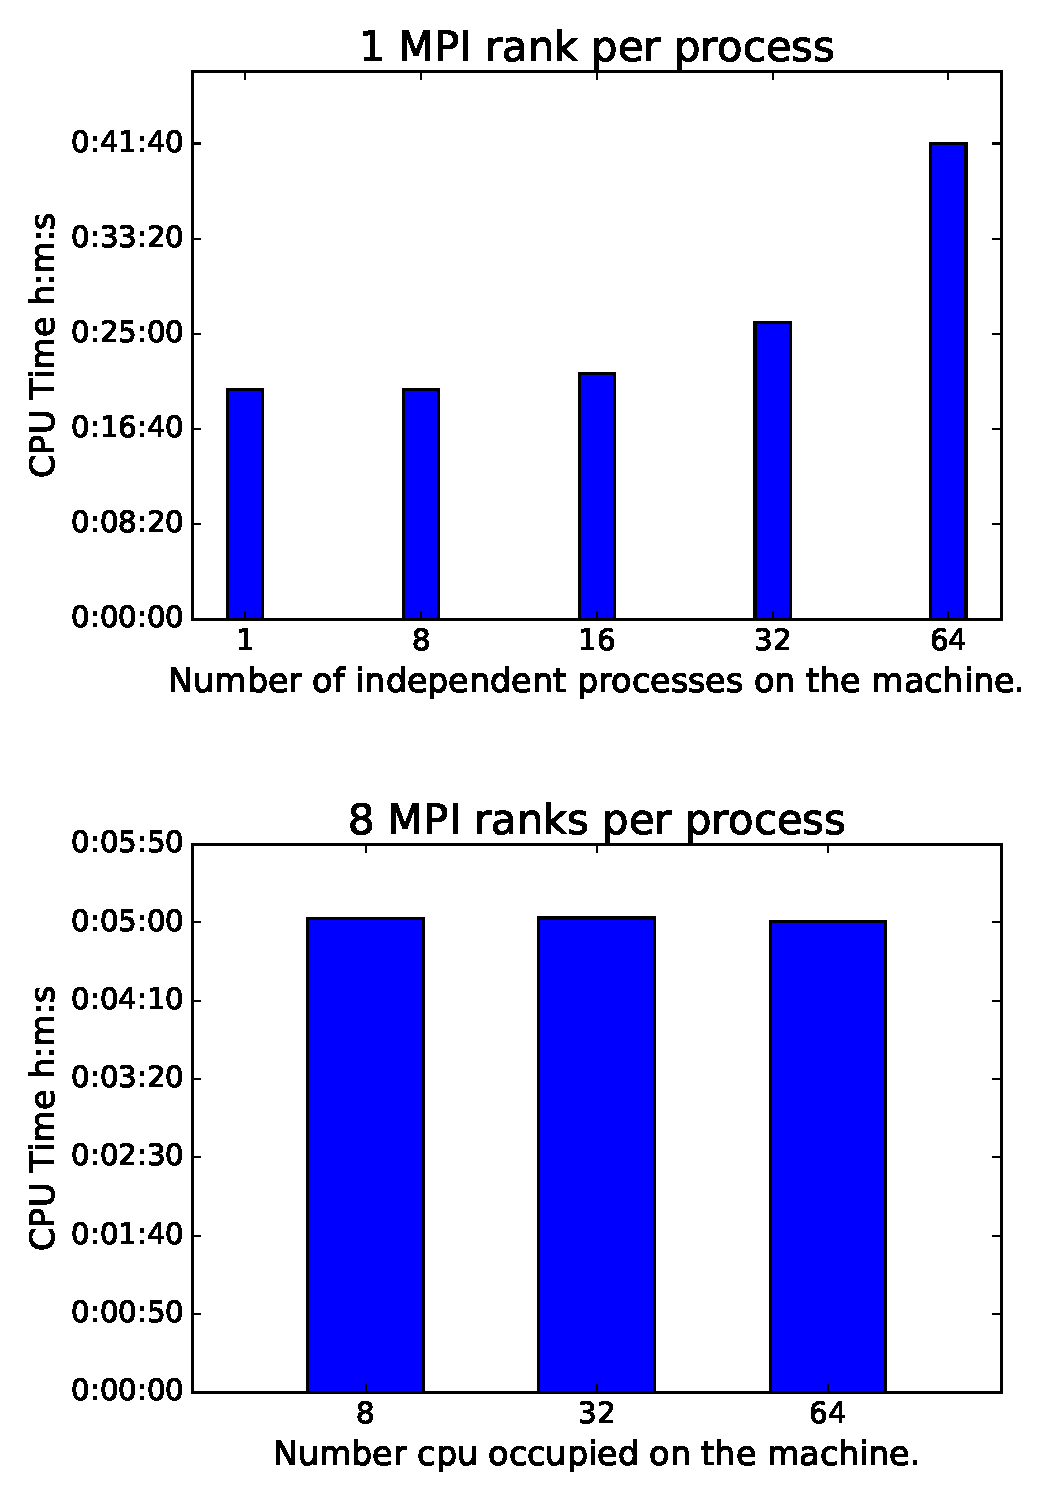
\includegraphics[width=0.7\linewidth]{sgiLoad.pdf}	
	\caption{asd}
	\label{fig:sgiLoad}
\end{center}
\end{figure}

To simulate different load conditions we ran simultaneously different instances of PWscf performing the same calculation.\footnote{Of the \CO system.}. Each instance of PWscf is completely independent.

In the first graph each instances was composed by a single MPI process, without threads. 
The execution time is plotted in function of the total number of independent processes running simultaneously on the machine.
The processes were equivalently spaced among the CPUs\footnote{Except for the first bar, the load of each node was the same.}.
Two aspects can be clearly seen.

First the execution time rises after 16 cores are simultaneously occupied, meaning at least half of the cores in each node.
When all the CPUs are occupied the execution time is more than doubled. 
We can say that the UV2000 performs poorly compared to the traditional cluster when multiple independent tasks have to be performed at the same time.

The second observation is that the execution time of the first and second bars are very close. 
In the first bar only a single CPU for on the whole machine is used; in the second bar a single CPU (the first one) for each node is used;
The fact that the times are the same suggests that each node behaves almost independently.

To confirm this speculation we raised the number of MPI ranks per PWscf instance to eight\footnote{The number of CPUs in a node.} and we performed three tests represented  in the second graph of figure \ref{fig:sgiLoad}.
The first bar occupies only one node per machine, the second half of the nodes and the third all of them.

The execution times are basically the same, hence we can say that every node behaves independently.

\begin{center}
\textit{Then the UV2000 machine can be used to perform simultaneously different independent calculations, provided that each node, or set of nodes, is used separately.}
\end{center}

The same results can be obtained with different numbers of MPI ranks per instance, see APPENDICE.
\mynotes{metti appendice}

\begin{framed}
After these preliminary tests, we decided to run every calculation always reserving the whole resource, being it a Galileo node or the whole UV2000 machine.
\end{framed}




\paragraph{Process migration (UV2000) : }

In modern multiprocessor architecture, even in a common desktop workstations, the Linux scheduler is used to migrate active processes from one CPU to another. 
In machine with a single shared memory controller  or with multiple controllers with uniform memory access time \footnote{UMA \textit{Uniform Memory Access} machines.}, the migration of a process doesn't have an impact on performances.
On NUMA machines instead, where the time to access a memory page depends on the page location withing the machine topology, this could negatively influence the performance of the code.
On the UV2000, memory allocation requested by a process is performed on the same node the process is running on. 
If the process is then migrated to another node the access time will increase at least by a factor of five.
The impact is mitigated by the NUMAlink behavior, which will migrate memory pages closer to the new process location (if available).

Another effect one must consider is that if an MPI job is launched on a subset of cores, i.e. requesting eight ranks, the ranks are randomly spread trough the whole machine.
Making a simple analogy, it would be equivalent to launch a single process on a different cluster node and expect the same performances.
If we introduce threads the scenario can get increasingly worse.
To obviate this problem a set of utilities developed by SGI can be used:

\texttt{omplace} is a command that forces the scheduler to maintain a process on the selected core, this feature is called \textit{process pinning}. 
\texttt{omplace} automatically takes care of threads placement and provides great flexibility on CPU placement.
In order to use \texttt{omplace} it is sufficient to prepend it to the MPI call.

For example:
\begin{verbatim}
	omplace -c 0-7 mpirun -np 8 pw.x
\end{verbatim}
will launch eight MPI ranks on the first eight processors.

Using threads 
\begin{verbatim}
	export OMP_NUM_THREADS=2
	omplace -c 0-7 mpirun -np 4 pw.x
\end{verbatim}
will launch an MPI rank on even cores and every rank will spawn two adjacent threads.
\mynotes{metti esempio da man omplace}

Although \texttt{omplace} can be used also with openMPI implementations, it works best with MPT.

\newpage







After this considerations we decided to perform all our tests in optimal conditions.
That are:
\begin{itemize}
	\item ``\textit{State of the art}" libraries and compilers
	\item Completely dedicated nodes. Meaning that on Galileo the whole node was reserved even if the computation was performed on a single CPU. This can be done using the PBS directive \texttt{select=1:ncpus:16:...}. On the UV2000 the while 64 core machine was reserved.
	\item On the UV2000, process are pinned using the \texttt{omplace} command. This command will prevent the migration of a process or thread from one CPU to another.
\end{itemize}


\begin{itemize}
	\item librerie open NO -> solo il meglio. State of the art for the architecture. Makefile delle due macchine.
	\item sempre a macchina scarica
	\item dlook, nodeinfo. QE si comporta bene, gestisce bene la memoria.
	\item MPT

\end{itemize}


\subsubsection{Strumenti}
\begin{itemize}

	\item profiling interno di QE
	\item scorep
\end{itemize}


\subsubsection{Metrics}
\begin{itemize}
	\item cpuTime
	\item wallTime (diskio = None)
	\item speedup
\end{itemize}


\section{Results}
\subsection{Dichiarazione di intenti}\label{sec:dichiarazionePoetica}
\begin{itemize}
	\item tuning QE indip da architettura (software)
	\item tuning QE dip da architettura 
	\item studio delle instabilita' numeriche. (iterazioni variabili)
\end{itemize}

\subsubsection{TiOH2}
IMPORTANTE: Spiega perche' hai usato TITANIA.

\subsubsection{Plots}
Per ogni sottosezione di sopra \ref{sec:dichiarazionePoetica} mettere da 6 a 8 grafici (AXES!) massimo.
Metti cerchio sui grafici dove IB spacca.


In fondo mettere i risultati per ogni molecola di size diverso.
	
Tutti i grafici che restano vanno a popolare l'appendice.

\section{Discussion and Conclusion}

\mynotes{Metti molecola organica}.

\mynotes{sarebbe bello patchare il codice per fargli tenere i core dell'algebra lineare tutti vicini! in modo che la comunicazione sulla numa sia localizzata! Hai tutto sugli appunti del 14/3 con Davide}

\mynotes{ci sono parti non parallelizzate fuori dai conti SCF, tipo il calcolo delle forze, c'e' spazio di miglioramento}
\mynotes{il numero di iterazioni scf cambia con il numero dei core per via di come viene valutato il criterio di convergenza.}
\mynotes{bisognerebbe dare piu' flessibilita' sulla posizione dei core dedicati alla diagonalizzazione.}




May the force be with you.

%In this work, we relate the insect concentration fluctuations to the
%dissipation of Milan University budget to catering companies.
%%
%We find it appropriate to name the present result ``{\em
%fluctuation-dissipation theorem}''.


%------------------------------------------------------------------
%  BIBLIOGRAPHY
%------------------------------------------------------------------
\clearpage
\addcontentsline{toc}{section}{Bibliography}
\begin{thebibliography}{9}

% note that the references must be listed in the same order as they are cited
% in the text above:

%\bibitem{Manini82} % standard format for a book:
%X. Manini and G. D'Annunzio,
%{\it Terra Vergine} (Springer-Verlag, Berlin, 1882).
%
%\bibitem{Jones55} % standard format for a journal article:
%M. Jones and J. Mones, J. Irreprod. Results {\bf 83}, 2322 (1955).
%
%\bibitem{Dragoni11}  % standard format for a thesis:
%D. Dragoni, {\it Interfacial layering of ionic liquids on solid surfaces},
%diploma thesis (University Milan, 2011),
%\url{http://www.mi.infm.it/manini/theses/dragoni.pdf}.

\bibitem{Atkins}
P. W. Atkins and R. S. Friedman,
Molecular Quantum Mechanics,
Oxford University Press, New York,
3rd Edition,
1997.

\bibitem{Attila}
A. Szabo, N. S. Ostlund,
Modern Quantum Chemistry: Introduction to Advanced Electronic Structure Theory,
Dover Pubblications, New York,
1996.

\bibitem{Dan}
D. Dan, Notes on General Chemistry,
Chapter 3.5, Many-electron atoms: Fermi holes and Fermi heaps,
W. H. Freeman Publisher,
2006.

\bibitem{Sakurai}
J. J. Sakurai,
Modern Quantum Mechanics,
Addison-Wesley,
Revised Edition,
1994.

\bibitem{Carati}
A. Carati, L.Galgani,
Appunti di Meccanica Razionale 1,
\url{http://users.mat.unimi.it/users/carati/#Didattica}.

\bibitem{Parr}
R. G. Parr, W. Yang,
Density Functional Theory of Atoms and Molecules,
Oxford University Press,
1989.

\bibitem{Basdevant}
J. L. Basdevant, J. Dalibard,
Quantum Mechanics,
Springer,
2005.


\bibitem{Thomas27}
L. H. Thomas, ``The calculation of atomic fields", Proc. Cambridge Phil. Soc. \textbf{23},542 (1927)

\bibitem{Fermi27}
E. Fermi,``Un Metodo Statistico per la Determinazione di alcune Priopriet\'a dell'Atomo", Rend. Lincei \textbf{6}, 602 (1927)

\bibitem{HK}
P. Hohenberg and W. Kohn, ``Inhomogeneous Electron Gas",  Physical Review \textbf{136} (3B): B864 (1964)

\bibitem{KS}
W. Kohn and L. J. Sham, ``Self-Consistent Equations Including Exchange and Correlation Effects". Physical Review \textbf{140} (4A): A1133 (1965)


\bibitem{Tanenbaum}
A. S. Tanenbaum, T. Austin,
Structured Computer Organization,
Sixth edition,
Pearson,
2012


\bibitem{Martin}
R. Martin, 
Electronic Structure,
Cambridge University Press,
2008.

\bibitem{Manini}
N. Manini, 
Introduction to the Physics of Matter,
2006,
\url{http://materia.fisica.unimi.it/manini/dida/Struttura_della_Materia_1.html}.


\bibitem{QE}
P. Giannozzi , S. Baroni , N. Bonini,``QUANTUM ESPRESSO: a modular and open-source software project for quantum simulations of materials", J. Phys.: Condens. Matter \textbf{21} (2009) 395502 (19pp)

\bibitem{QEManual}
``User's Guide for Quantum ESPRESSO", \url{http://www.quantum-espresso.org/wp-content/uploads/Doc/user_guide.pdf}.

\bibitem{MPI}
``MPI :A Message-Passing Interface Standard", \url{http://www.mpi-forum.org/docs/mpi-3.1/mpi31-report.pdf}

\bibitem{OMP}
``OpenMP Application Programming Interface", \url{http://www.openmp.org/mp-documents/openmp-4.5.pdf}

\bibitem{FFTW}
``Fast Fourier Transform in the West" project page, \url{http://www.fftw.org/}.


\bibitem{Marx}
D. Marx, J. Hutter,
Ab initio Molecular Dynamics,
Basic Theory and Advanced Methods,
Cambridge University Press,
2009.

\bibitem{Davidson}
E. R. Davidson, ``Super-Matrix Methods", Comput. Phys. Comm., \textbf{53} 49 (1989)

\bibitem{Johnson}
D. D. Johnson, ``Modified Broyden’s method for accelerating convergence in self-consistent calculations", Phys. Rev. B \textbf{38}, 12807 (1988)

\bibitem{Galileo}
\url{http://www.top500.org/system/178549},
\url{http://www.hpc.cineca.it/hardware/galileo}.

\bibitem{MPT}
Full specification of the Message Passing Toolkit can be retrieved using the command : man MPT.

\end{thebibliography}


\end{document}


